\RequirePackage[2020-02-02]{latexrelease}  
\documentclass[12pt]{zHenriquesLab-StyleBioRxiv}
\usepackage{relsize, multirow, xcolor,xargs, placeins}
\usepackage{amsfonts, amsmath, amsthm, amssymb, siunitx} % For math fonts, symbols and environments
\usepackage{environ, etoolbox}
\usepackage{lineno} 
\definecolor{sunyGray}{RGB}{131,134,135} 
\definecolor{sunyBlue}{RGB}{0,76,147}     
\newcommandx{\cyansub}[1]{\large\textcolor{sunyBlue} \noindent \textcolor{sunyBlue} {\noindent\textbf{#1}}}                             
\newcommand{\myemph}[1]{\textbf{\textit{#1}}}
\newcommand{\Ga}{\mbox{Ga}} 
\newcommand{\N}{\mathcal{N}} 
\newcommand{\E}{\mbox{E}}                                                                                                                                                           

\newcommand{\V}{\mbox{V}}




\newcommand\fref[1]{\normalsize{\textbf{\textit{Fig.\,\ref{#1}}}}\normalsize{}}                                                                                                    
\newcommand\dref[2]{\normalsize{\textbf{\textit{Fig.\,\ref{#1}#2}}}\normalsize{}}                                                                                                  
\newcommand\sref[1]{\normalsize{\textbf{\textit{Supplementary Fig.\,\ref{#1}}}}\normalsize{}}                                                                                       
\newcommand\stref[1]{\normalsize{\textbf{\textit{Supplementary Table\,\ref{#1}}}}\normalsize{}}                                                                                       



\setlength\parindent{0.50cm}
\setlength{\parindent}{0cm}
\setlength{\parskip}{0.4\baselineskip} 

\leadauthor{Souaiaia} 
\begin{document}
\title{Striking Departures from {\color{red}{Common Polygenicity}} in the Tails of Complex Traits}
\shorttitle{Tails}
\author[1,\Letter*]{Tade Souaiaia}
\author[2*]{Hei Man Wu}
\author[2,3]{Anil P.S. Ori} 
\author[2]{Shing Wan Choi} 
\author[2]{Clive J. Hoggart}
\author[2,\Letter]{Paul F. O'Reilly}
\affil[1]{Department of Cellular Biology, Suny Downstate Health Sciences University, Brooklyn, NY, USA}
\affil[2]{Department of Genetics and Genomic Sciences, Icahn School of Medicine, Mount Sinai, NY, NY, USA}
\affil[3]{Department of Psychiatry, Amsterdam UMC, University of Amsterdam, Amsterdam, The Netherlands} 
\affil[*]{These authors contributed equally to this work}
\onecolumn \maketitle
\vspace*{-5mm}
%\begin{corrauthor} \texttt{\small tade.souaiaia\at downstate.edu, clive.hoggart\at mssm.edu, paul.oreilly\at mssm.edu} \end{corrauthor}
\begin{corrauthor} \texttt{\small tade.souaiaia\at downstate.edu, paul.oreilly\at mssm.edu} \end{corrauthor}
\vspace*{-2mm}
\noindent\textcolor{sunyGray}{\rule{17.25cm}{1mm}}
\linenumbers
%%%%%%%%%%%%%%%%%%%%%%%%%%%%%%%%%%%%%%%%%%%   END PREAMBLE  %%%%%%%%%%%%%%%%%%%%%
% 
%  PREV: PREAMBLE, NEXT: ABSTRACT
%  PREV: PREAMBLE, NEXT: ABSTRACT
%  
% Sanjak   Fig  
%%%%%%%%%%%%%%%%%%%%%%%%%%%%%%%%%%%%%%%%%%%%%%%%%%%%%%%%%%%%%%%%%%%%%%%%%%%%%%%%%
%%%%%%%%%%%%%%%%%%%%%%%%%%%%%%%%%%%%%%%%%%%   ABSTRACT  %%%%%%%%%%%%%%%%%%%%%%%%%
%%%%%%%%%%%%%%%%%%%%%%%%%%%%%%%%%%%%%%%%%%%%%%%%%%%%%%%%%%%%%%%%%%%%%%%%%%%%%%%%%

\begin{abstract} %\normalsize
\noindent\cyansub{Abstract}$\,$ 
{\color{red}{The relative contribution of common and rare genetic variants to complex trait heritability is of key biological, pharmaceutical and clinical importance. Yet how these contributions vary across the trait distribution – and how this differs between traits subject to different selective pressures – is underexplored. Here, we introduce a novel polygenic score-based method (“POPout”) to detect deviations in common-variant architecture across the trait continuum. Applying POPout to 74 quantitative traits, we uncover widespread departures from common polygenicity in one or both tails of most of the traits, consistent with distinct enrichments of high-effect, rare alleles. We demonstrate replication of these results across ancestries, cohorts, repeat measures, and using an independent family-based approach. While our methods do not rely on rare variant discovery, which remains limited by statistical power, we find direct support for inferred enrichments using exome and whole genome sequence data. Moreover, simulations demonstrate that traits under stabilising selection are expected to have tails enriched for high-effect, rare alleles, and we find empirical evidence of ongoing selection consistent with our findings. Finally, trait tails with inferred enrichment of high-effect, rare alleles are associated with reduced fecundity, advanced paternal age, and decreased accuracy of polygenic scores. This work has broad implications for rare variant discovery, genetic prediction, the study of selection in humans, and for the relative importance of common and rare variants to complex traits and diseases.} 
    }
\end {abstract}
%\vspace*{-5mm}
%\noindent\textcolor{sunyGray}{\rule{17.25cm}{1mm}}
%\vspace*{-7mm}
%%%%%%%%%%%%%%%%%%%%%%%%%%%%%%%%%%%  END ABSTRACT  %%%%%%%%%%%%%%%%%%%%%%%%%%%%%
% 
% 
% 
% 
% 
% 
% 
% 
% 
% 
% 
% 
% 
% 
% 
% 
% 
% 
% 
% 
% 
% 
% 
% 
% 
% 
%%%%%%%%%%%%%%%%%%%%%%%%%%%%%%%%%%%%%%%%%%%%%%%%%%%%%%%%%%%%%%%%%%%
%%%%%%%%%%%%%%%%%%%%%%%%%%%%%%   INTRO  %%%%%%%%%%%%%%%%%%%%%%%%%%%
%%%%%%%%%%%%%%%%%%%%%%%%%%%%%%%%%%%%%%%%%%%%%%%%%%%%%%%%%%%%%%%%%%%
\section*{Introduction}  \label{sec:intro}  
Genome-wide association and sequencing studies have identified many thousands of common and rare variants associated with a 
wide range of complex traits \cite{Abdellaoui2023,Flannick2019,Singh2022}. The number of variants 
identified is now so large that a complete picture of the genetic architecture of 
many complex traits is starting to emerge. Recent publications illustrate all known 
variants for a trait or disease on a spectrum of allele frequency versus effect size, producing a 
characteristic "trumpet" shape \cite{Yengo2022,Corte2023}{\color{red}{, in which identified rarer variants have exponentially larger effects. These effects are sometimes so large relative to those of common alleles that they cause extreme trait values on most genetic backgrounds.}} For example, mutations in ACAN usually result in short stature \cite{vanDerSteen2017}, in LEP that typically cause leptin 
deficiency and severe early onset obesity \cite{Saeed2015}, and in HNF1A 
that produce large deviations in glucose homeostasis and early-onset diabetes \cite{Miyachi2022}. 
Therefore, it is already known that there are single alleles of sufficient effect size 
to generate extreme trait values in individuals. Moreover, Fiziev et al. \cite{Fiziev2023} 
demonstrated that rare polygenic risk scores (PRS), {\color{red}{based on an aggregate of rare allele effects inferred using their PrimateAI-3D algorithm, were particularly predictive for individuals with extreme trait values. Rare alleles with dramatic effects on complex disease have also been identified, such as in LPA on cardiovascular disease, in the APP and PSEN genes that cause Alzheimer’s disease, and cumulative loss-of-function mutations associated with more severe forms of schizophrenia and autism.}}

{\color{red}{Based on the existence of rare alleles that can alone generate extreme trait values, and growing evidence that stabilising selection is a pervasive driver of complex trait genetic architecture, we hypothesise that stabilising selection on some traits may be strong  enough to have produced marked enrichments of high-effect, rare alleles in the tails of continuous, complex traits. To test this hypothesis, we develop methods based on contrasting expectations under neutrality and strong selection (Fig.1). For traits under no selection, we expect independence between allele frequencies and effect sizes (Fig.1a), resulting in a consistent contribution of common and rare variants to heritability across the trait continuum (Fig.1b), a linear relationship between trait values and common PRS (Fig.1c; trait quantiles shown here), and regression-to-the-mean among siblings of individuals with extreme trait values. For traits under strong selection, we expect rare alleles of far larger effect than common alleles (Fig.2a), resulting in rare-variant heritability that is exponentially larger in the tails (Fig.2b), common PRSs in the tails that are less extreme than expected on average (Fig.2c), and siblings of individuals with extreme trait values (when caused by de novo mutations here) having trait values reflective of the background trait distribution.}}






%%%%%%%%%%%%%%%%%%%%%%%%%%%%%%%%%%%%%%%%%%%%%%%%%%%%%%%%%%%%%%%%%%%%%%%%
%%%%%%%%%%%%%%%%%%%%%%%%%%%%  FIGURE 1 %%%%%%%%%%%%%%%%%%%%%%%%%%%%%%%%%
%%%%%%%%%%%%%%%%%%%%%%%%%%%%%%%%%%%%%%%%%%%%%%%%%%%%%%%%%%%%%%%%%%%%%%%%
%\vspace*{-2mm} 
%\FloatBarrier 
\begin{figure}[!h] 
\centering 

\includegraphics[trim=0cm 0cm 0cm 0cm, clip, width=0.98\linewidth]{Figures/Fig1.pdf} 
\caption{{\textbf{Two polygenic models of complex trait genetic architecture.} 
In the polygenic model with no selection: \textbf{a}, the minor allele frequency (MAF) and effect size of 
variants affecting the trait are uncorrelated, \textbf{b}, 
common and rare variants are uniformly distributed across the trait continuum and common variants explain more heritability, 
\textbf{c}, the trait and polygenic score have a linear, monotonic relationship, and 
\textbf{d}, siblings of individuals in the tails of the trait distribution also show low/high trait values, 
with regression-to-the-mean dependent on trait heritability \cite{Souaiaia2024}. 
The hallmark of this model is that polygenic architecture predominates the entire trait distribution. 
In the polygenic model with strong selection (here, stabilising selection): 
\textbf{e}, there is a strong relationship between MAF and effect size, whereby only rare alleles have large effect, 
\textbf{f}, common variants explain more heritability overall, but rare variants contribute more in the tails, 
\textbf{g}, the polygenic score (derived from common variants) regresses to the mean in the trait tails due to 
enrichment of high-impact rare alleles not included in the polygenic score, \textbf{h}, assuming selection is so 
strong to produce tails characterised by \emph{de novo} architecture, then siblings of individuals in the trait tails 
have trait values drawn from the background distribution. The hallmark of this model is that polygenic architecture 
prevails across most of the trait distribution, except for the tails where rare-variant architecture predominates. 
These models illustrate two extremes of selection, neither of which will be applicable for most traits (indeed recent work suggests polygenicity may be caused by selection \cite{Oconnor2019}); however, most complex traits should be captured by an intermediate model that lies somewhere between these two extremes.}}
\label{fig1} 
\end{figure} 
%\FloatBarrier 


{\color{red}{In this study, we develop population-based and family-based methods to interrogate the tail architecture of complex traits, we investigate the role of selection in shaping this architecture, and we consider the implications of our observations on PRS accuracy and rare-variant discovery. First, we introduce the PRS-On-Phenotype outlier (“POPout”) test, a novel method that uses PRS to detect deviations in common polygenic expectations in the tails of trait distributions (e.g. in the lowest and highest 1\% of LDL, BMI, glucose).}} The premise of the POPout test is that a PRS derived from common variants should exhibit a positive, linear relationship with its corresponding trait in the absence of selection and large, unaccounted environmental effects (Fig.1c). However, under strong selection, high-effect, rare alleles are concentrated in the trait tails and the common PRS regresses towards the mean in these extremes (Fig.1g). We first apply POPout to 74 quality-controlled quantitative traits in individuals of European ancestry from the UK Biobank, followed by replication in individuals of multiple ancestries from the UK Biobank, in individuals with repeated measures, and in the US-based All of Us cohort. Next, we use an independent approach that leverages sibling trait variability to infer the genetic architecture of trait tails (Fig.1d, Fig.1h) in over 17k sibling pairs from the UK Biobank. This sibling-based approach provides complementary evidence to POPout, since it utilises non-genetic family data to infer tail architecture. Across these methods and cohorts, we observe widespread and substantial departures from common polygenic expectations in trait tails (Fig.2, Fig.3). {\color{red}{We find direct evidence for the role of rare variants in these departures from common polygenicity using published exome study results and by incorporation of rare variants – identified through our own whole genome sequence study analyses – into the PRSs.} To verify natural selection as a driver of these observations, we extend a method that uses lifetime reproductive success to infer ongoing positive, negative, and stabilising selection, finding consistency between the type of selection inferred and the trait tail(s) that appears to be under selection according to our POPout results. Supporting this, simulations using the forward-in-time simulator SLiM, show that stabilising selection results in POPout effects in both tails, whereas traits simulated under neutrality display no such effects. {\color{red}{Our findings highlight the distinct nature of genetic architecture in the tails of complex traits, emphasize the role of selection in the causes of phenotypic extremes, and imply strategies for increasing the accuracy of genetic prediction of complex traits and disease.}} 


%%%%%%%%%%%%%%%%%%%%%%%%%%%%%%%%%%%%%%%%%%%%%%%%%%%%%%%%%%%%%%%%%%%%%%%%%%%%%%%
%%%%%%%%%%%%%%%%%%%%%%%%%%%%%%%%%%%   END INTRO %%%%%%%%%%%%%%%%%%%%%%%%%%%%%%%
%%%%%%%%%%%%%%%%%%%%%%%%%%%%%%%%%%%%%%%%%%%%%%%%%%%%%%%%%%%%%%%%%%%%%%%%%%%%%%%   
% 
% 
% 
% 
%  PREV: INTRO, NEXT: RESULTS 
% 
% 
% 
% 
% 
% 
% 
% 
% 
%
% 
% 
%  PREV: INTRO, NEXT: RESULTS 
% 
% 
% 
% 
% 
% 
% 
% 
%  PREV: INTRO, NEXT: RESULTS 
% 
% 
% 
% 
% 
% 
% 
% 
% 
%%%%%%%%%%%%%%%%%%%%%%%%%%%%%%%%%%%%%%%%%%%%%%%%%%%%%%%%%%%%%%%%%%%%%%%%%%%%%%%%   
%%%%%%%%%%%%%%%%%%%%%%%%%%%%%%%%%%%%%%%%%%%   RESULTS - START  %%%%%%%%%%%%%%%%%
%%%%%%%%%%%%%%%%%%%%%%%%%%%%%%%%%%%%%%%%%%%%%%%%%%%%%%%%%%%%%%%%%%%%%%%%%%%%%%%%
{\color{black}{
\section*{Results} \label{sec:results} 
\subsection*{Widespread POPout effects} 
Here} we first investigate how genetic architecture 
varies across the trait continuum in a range of 
quantitative traits using UK Biobank (UKB) 
genotype-phenotype data \cite{Bycroft2018}. We consider traits 
from the broad UKB trait categories of \emph{Biomarkers}, 
\emph{Physical Measures}, \emph{Touchscreen Questionnaire}, and \emph{Cognitive Function}. 
After quality control (QC) steps (see Methods), to ensure, for example, 
that the traits selected for analysis are heritable, approximately normally distributed and 
sufficiently independent, 74 traits remain for analysis. 
To limit the contribution of environmental factors, we 
residualised the traits with a range of covariates, including 
age, sex, smoking, alcohol intake and diabetes status, and 
removed individuals with cancer diagnoses or who 
were pregnant, as well as individuals on statins or on 
insulin medication within the biomarker category. 
After standard QC of the genotype data,
there were 369,132 unrelated individuals of European (EUR)
ancestry available for the primary analysis, with SIBLINGS AND 
INDIVIDUALS OF OTHER ANCESTRIES RETAINED FOR 
REPLICATION ANALYSES (SEE METHODS). 

We developed a method (see Methods) that leverages polygenic risk scores (PRS), 
derived from common variants, to infer DEVIATIONS IN COMMON POLYGENICITY  
in the tails of quantitative traits. In standard PRS
analyses \cite{Choi2020}, PRS is a predictor of outcome, 
with results often displayed as a quantile plot showing 
higher values (or odds ratio) of the outcome with increasing 
PRS quantiles \cite{Khera2018,Khera2019}. Here we invert this 
relationship, so that trait is a predictor of PRS, displaying 
results as trait quantiles on the X-axis and PRS on the Y-axis.
This simple reversal of the usual relationship enables us to 
investigate how the PRS varies along the trait continuum. 
Under a null hypothesis OF A POLYGENIC TRAIT UNDER NO OR WEAK SELECTION,  
with environmental factors adjusted or jointly 
normally distributed, we expect a linear relationship between 
the trait and PRS (\dref{fig1}{c}). In contrast, if the tails are enriched for HIGH-EFFECT rare alleles, 
not included in the PRS derived from GWAS on 
common variants, then the average PRS in the lower and upper 
quantiles will regress to the population mean PRS (\dref{fig1}{g}). 
We formally tested for deviations from the LINEAR expectations OF 
OUR NULL HYPOTHESIS by performing $t$-tests on the residuals 
of a regression of PRS on trait. Each of the middle 80 trait centiles 
were tested as a QC step, while the analysis test - which we refer to 
as the “PRS-On-Phenotype outlier test”, or POPout test - 
is applied to the lower and upper trait centiles (see Methods). 
The POPout test is applied to the bottom and top 1\% of 
trait values here since these quantiles are considered sufficiently 
extreme to be subject to selection, given the typical prevalence of 
complex disease, yet broad enough for sufficient sample size. 
%%%%%%%%%%%%%%%%%%%%%%%%%%%%%%%%%%%%%%%%%%%%%%%%%%%%%%%%%%%%%%%%%%%%%%%%
%%%%%%%%%%%%%%%%%%%%%%%%%%%%  FIGURE 2 %%%%%%%%%%%%%%%%%%%%%%%%%%%%%%%%%
%%%%%%%%%%%%%%%%%%%%%%%%%%%%%%%%%%%%%%%%%%%%%%%%%%%%%%%%%%%%%%%%%%%%%%%%
%\FloatBarrier 
\begin{figure}[!h] \centering 
\includegraphics[trim=0cm 0cm 0cm 0cm, clip, width=\linewidth]{Figures/Fig2.pdf} 
\caption{{{\bf Population-based POPout analyses.}
\textbf{a,} Trait quantiles (1\% increments) plotted against mean
PRS value for four traits with different POPout
characteristics.  Expected PRS (orange) calculated from regression of PRS on trait. 
\textbf{b,} 
POPout results across 74 QC’ed traits in UKB EUR data. 
Effects with 95\% confidence intervals shown. 
\textbf{c,} 
Odds ratio corresponding to the lowest/highest 1\%/25\% of the trait as index PRS 
quantile versus the central PRS quantile. Orange dashed line is expected performance 
assuming infinitesimal model (shaded area highlights the difference with observed). 
\textbf{d,}
POPout effect sizes from UKB EUR analysis (of b) plotted against replication POPout 
effect sizes for upper and lower tails of all overlapping traits. 
Correlation between UKB EUR and replication effect sizes calculated using Pearson.
}}\label{fig2} 
%\vspace*{-5mm} 
\end{figure}
%\FloatBarrier
%

We applied the POPout test to the 74 traits in the UK Biobank, 
randomly splitting the sample of 369,132 individuals into two halves, 
in which a GWAS is performed in the first half, the results of which 
are used to derive and train PRSs in the second half, which is used 
for the POPout analyses. {\color{red}{The POPout test is performed in the same 
sample in which PRSs are trained, resulting in a conservative bias in 
POPout effects that we consider worthwhile to optimise sample 
size for testing in the tails (see Methods)}}. \dref{fig2}{a}  displays PRS-on-trait quantile plots corresponding 
to four of the traits that illustrate different types of 
observed relationships. Phosphate shows a relationship that 
follows LINEAR expectations (orange line) closely. 
Haemoglobin concentration shows a strong departure from 
LINEAR expectations in the lower tail, corresponding 
to a POPout effect size of 0.37 ($P = 2.6 \times 10^{-36}$), 
consistent with strong enrichment of HIGH-EFFECT, rare alleles in the lower 
tail, while red blood cell distribution width shows a strong 
regression-to-mean of PRS in the upper tail (POPout effect: 
0.5; $P = 5.7 \times 10^{-60}$), consistent with a concentration
of HIGH-EFFECT, rare alleles residing in individuals of 
the upper tail. Sitting height shows strong POPout effects in both 
tails (lower tail $P = 3.5 \times 10^{-60}$, upper 
tail $P = 4.3 \times 10^{-25}$), consistent with HIGH-EFFECT, rare allele 
enrichments in both tails CAUSED BY stabilising selection. The four 
traits included in \dref{fig2}{a}  were selected because they provide clear illustrations 
of the different types of relationship and are not reflective of 
the general results. 

In the full POPout analysis of 74 traits, 
68 traits had significant (FDR$<5\%$) POPout effects in one or both 
tails, suggestiVE OF pervasive - AND SOMETIMES STRIKING - departures from COMMON polygenicITY 
in the tails of complex traits in general (\dref{fig2}{b}, \stref{sup2a}). 
Of the 107 tails with significant 
POPout overall, 97 CORRESPONDED TO POSITIVE POPOUT 
EFFECTS, CONSISTENT WITH OUR HYPOTHESIS OF RARE 
VARIANT TAIL ENRICHMENT. The 10 significant negative POPout effects could be a result 
of epistatic OR GENE-BY-ENVIRONMENT effects (see Discussion).

To exemplify the impact of these observed deviations from 
polygenic expectations, we emulated PRS prediction of 
case/control status for diseases hypothetically diagnosed 
in individuals with low haemoglobin and high red blood cell 
distribution width, with prevalences of 1\% and 25\% (\dref{fig2}{c}). 
While prediction of case/control status using the trait PRS 
is as expected (orange dashed line) for a disease prevalence 
of 25\%, the PRSs underperform substantially for both 
traits for disease prevalence 1\%. For haemoglobin, the mean 
odds ratio (OR) for individuals in the bottom 5\% of PRS is 
expected to be 3.7 but is in fact 1.8, while, for red blood 
cell distribution width, the mean OR for individuals 
with top 5\% PRS values is 1.8 instead of an expected 4.1.
%
\subsection*{Replication of POPout effects} \label{sec:res1}
Here we performed three different forms of replication to test the generalizability of our primary 
findings that used UKB European ancestry data. In each replication dataset, 
we only included traits that passed our POPout QC (see Methods) and have sample size 
over 5k individuals based on inferred power (see \sref{sup_rep}). First, 
to investigate if POPout effects of the primary analysis are due to residual 
non-genetic factors not captured by our QC or covariate adjustments, we repeated 
the analysis in a held-out sample of individuals that had traits measured at 
baseline and at approximately 5-year follow-up. By taking mean values of the 
two repeat measures, the impact of transient, environmentally influenced factors, 
such as infections, short-term medication use, or diet, should be minimised. 
This ‘UKB Repeated’ analysis, performed on up to $\sim$15k individuals across the 
50 (of 63 overlapping) traits that passed QC, showed a strong and 
significant ($R=0.71$, $P=2.3 \times 10^{-16}$) correlation with the results 
of the primary analysis (\dref{fig2}{d}), suggesting genetic contribution to the 
observed POPout effects of the primary analysis. Next, we investigated the generalizability 
of our findings to a held-out sample of UKB multi-ancestry individuals (see Methods). 
This ‘UKB Multi-Ancestry’ analysis, performed on up to $\sim$22k individuals across the 
54 traits that passed QC, produced highly correlated and significant 
replication ($R=0.63$, $P=3.7 \times 10^{-13}$) of the primary results (\dref{fig2}{d}). 
Finally, we apply the same approach to European ancestry individuals from the 
US-based All of Us data \cite{Bick2024} to evaluate the generalizability to a matched-ancestry 
sample but from a clinical-based cohort from a different continent, with different 
collection and assaying procedures, and a different healthcare system and set of 
environmental factors. This ‘All of Us’ analysis, performed on up to $\sim$127k individuals 
across the 28 (of 33 overlapping) traits that passed QC, also showed strong replication (\dref{fig2}{d}) of the primary 
analysis results ($R=0.59$, $P=1.6 \times 10^{-6}$). 
See Supplementary Material (\sref{sup_rep}) for a full breakdown of all replication analyses. 
%
%
\subsection*{Tail architecture inferred by siblings} 
Next, we leverage information about tail architecture that can be derived 
from family trait data. We have developed a method \cite{Souaiaia2024} that evaluates trait data in large 
samples of siblings to infer genetic architecture in the tails of quantitative traits. 
This provides an alternative, complementary approach to infer tail architecture 
from independent, family-based, non-genetic data. 
The intuition of the approach (\dref{fig3}{a}) is that individuals with extreme 
trait values have siblings whose trait values reflect the architecture in the tails, 
such that under: (1) polygenic architecture: siblings have high but less extreme trait 
values, (2) \emph{de novo} architecture: siblings have trait values reflective of the general 
population, (3) Mendelian architecture (i.e. due to rare, high-impact alleles that segregate 
in families): siblings either have similarly extreme trait values or have trait values that reflect the general population.

Having established theoretical expectations of sibling 
similarity according to genetic architecture, we developed 
tests to distinguish between these three possibilities \cite{Souaiaia2024} , 
which we extend here to a joint test, which we refer to as 
STANDout (Methods). STANDout infers general departures from polygenic expectations 
in trait tails from trait-only data and is powered to identify 
tail architecture enriched for large-effect, rare alleles 
(that can cause individuals to ‘stand out’ from their siblings for given traits), 
assuming environmental factors are adjusted or jointly normally distributed.
% backman 
%%%%%%%%%%%%%%%%%%%%%%%%%%%%%%%%%%%%%%%%%%%%%%%%%%%%%%%%%%%%%%%%%%%%%%%%
%%%%%%%%%%%%%%%%%%%%%%%%%%%%  FIGURE 3 %%%%%%%%%%%%%%%%%%%%%%%%%%%%%%%%%
%%%%%%%%%%%%%%%%%%%%%%%%%%%%%%%%%%%%%%%%%%%%%%%%%%%%%%%%%%%%%%%%%%%%%%%%
%\FloatBarrier
\begin{figure}[!h] 

\includegraphics[trim=0cm 0cm 0cm 0cm, clip, width=\linewidth]{Figures/Fig3.pdf} 
\caption{{{\bf Tail architecture inferred from siblings.}
\textbf{a,} 
Schematic of relationships between sibling trait values under tails governed by polygenic (grey), 
\emph{de novo} (red) and Mendelian (purple) architecture, where Mendelian here refers to rare (but not \emph{de novo}) 
high-impact alleles segregating in families. 
\textbf{b,} 
Index sibling trait quantile (1\% increments) plotted against mean trait 
value of other (conditional) sibling for the four traits selected with 
different POPout characteristics (see Fig.2a). 
\textbf{c,} POPout $P$-values plotted against STANDout $P$­-values for the 74 traits. Correlation and significance 
calculated using Pearson. 
\textbf{d,} LD score regression \cite{BulikSullivan2015} SNP-estimated heritability plotted against heritability estimated 
from sibling pair trait similarity \cite{Souaiaia2024}.
}} \label{fig3} \end{figure} 
%\FloatBarrier
%
%
%

The UK Biobank (UKB) includes over 17k sibling pairs of European ancestry available for our STANDout analyses, 
none of which were included in our population-based analyses. There were too few sibling pairs from the 
multi-ancestry sample for a sufficiently powered multi-ancestry sibling analysis. 
Data across all 74 traits were available for analysis. Replicating our POPout analysis, 
our STANDout analysis showed no departure from polygenic expectations for phosphate, showed 
a significant lower tail STANDout effect for haemoglobin concentration ($P_{lower}=2 \times 10^{-5}$), a 
significant upper tail STANDout effect for red blood cell distribution width ($P_{upper}=4 \times 10^{-4}$), 
and significant effects in both tails for sitting height 
($P_{lower}=7 \times 10^{-4}$, $P_{upper}=3 \times 10^{-8}$; see \dref{fig3}{b} and \dref{fig2}{a} for comparison). 
More broadly, our sibling-based STANDout analyses replicated our population-based POPout analyses across 
the 74 traits well (\dref{fig3}{c}; $R = 0.66$, $P = 3 \times 10^{-20}$). This is reassuring given that the 
two methods use such orthogonal approaches and types of data. Further reassurance of the validity of our 
sibling-based method is provided by the strong correlation ($R = 0.81$, $P = 2 \times 10^{-9}$) between 
SNP-based heritability ($h^2$), estimated by the popular LD score regression approach~\cite{BulikSullivan2015}, 
and the sibling-based $h^2$ estimated as a key parameter in the STANDout approach \cite{Souaiaia2024}  (\dref{fig3}{d}).

%
{\color{red}{
\subsection*{The role of rare variants}
In previous sections, we observed and replicated widespread 
departures from common polygenic expectations in the tails of quantitative 
traits. Here, we investigate direct evidence for rare variant enrichment 
underlying these patterns from whole exome sequence (WES) and whole 
genome sequence (WGS) data.}} Backman et al. \cite{Backman2021} conducted 
the most comprehensive trait-wide analysis of UK Biobank 
WES data to date, and here we utilise their 
results to investigate whether traits with significant POPout 
effects are associated with a greater number of significant 
exome variants (or ‘hits’), with effects in the expected 
direction. Considering our four example traits, phosphate has
two exome hits with positive and four with negative 
effect sizes, haemoglobin concentration has eight with 
positive and twelve with negative effect sizes, red blood 
cell distribution width has twenty-eight with positive and 
five with negative effects, and sitting height has ten with 
positive and twenty with negative effects (\dref{fig4}{a}). 
Across the 74 traits, we found that POPout effect sizes from 
our primary analysis are significantly positively 
correlated ($R=0.35$, $P=2\times10^{-5}$) with the 
number of exome hits with effects in the direction 
corresponding to the tail of the POPout 
effect (\dref{fig4}{b}). 

{\color{red}{
Next, we performed our own WGS analyses of the UK Biobank data. We 
performed GWASs of rare variants across the 74 traits in the same individuals 
used for the common-variant GWAS of our primary POPout analyses (Fig.2). We 
restricted our analyses to moderately rare variants (1$\%$ > MAF > 0.01$\%$) to 
allow single-variant testing of UKB SNPs and robust integration wit our common-variant
PRSs. We computed rare PRSs using genome-wide significant variants ($P < 1X10^{-11}$) 
with MAF between 1\% and 0.1\% and also between 0.1\% and 0.01\% and we combined 
these with the previously computed common PRSs to investigate whether the addition of moderately 
rare variants reduces POPout signal (Fig.4c). Among 68 traits tails with significant POPout effects 
and at least one significant rare variant, 49 had reduced POPout effect (Binomial test P=6.5x10^{-5}$), 
7 had significantly reduced POPout ($P < 0.05$) with a mean reduction in POPout effect of 27\% and 0 
had significantly increased POPout (Fig.4d). In Supplementary Table X, we report the PRS $R^{2}$ and 
odds ratio (OR) for individuals with elevated PRS (for hypothetical cases defined in the trait tails; see Methods), 
for each trait before and after inclusion of rare variants. While the impact of the rare variants on PRS R2 is 
modest (mean relative R2 increase = X), their impact on ORs is substantial (mean relative OR increase = Y), 
highlighting the over-sized impact of rare variants on trait tails. Furthermore, reduced POPout across the 
traits is mostly due to the rare variants (i.e. 0.1\% > MAF > 0.01\%), whereas as increased POPout is mostly 
due to the less rare variants (i.e. 1\% > MAF > 0.1\%). This suggests that much of the residual POPout effect
may be caused by ultra-rare variants, consistent with results from our simulations (see next section) and 
other work indicating a larger contribution from ultra-rare variants (REFs). Moderately rare variants sill to be 
identified by larger studies are likely to be another important contributor. Next we derive estimates of high-effect 
rare-variant heritability based on the size of POPout effect and PRS $R^2$ (see Methods). Fig.4d shows these 
$h^{2}$ estimates before and after inclusion of rare variants, computed both as an upper bound by assuming that 
rare variants explain the entire POPout effect and also assuming that their contribution is proportional to the trait 
heritability. Upper bound rare-variant heritability has range 0.03 < $h^{2}$ < 0.21 (mean 0.12) for 15 of the 16 
traits (see below regarding the outlier trait: age of menopause), while that incorporating contribution from 
non-genetic factors has range 0.01 < $h^{2}$ < 0.11 (mean 0.06). These estimates are somewhat higher than 
the "burden heritability" estimates of Weiner et al, although this may be explained by our estimates accounting 
for all types of variant genome-wide, rather than only SNPs within exomes. Age of menopause was an extreme 
outlier in our estimates of rare-variant heritability, which could reflect far stronger selection acting on this trait 
because of its direct role in reducing fecundity. In the next section, we investigate how selection shapes trait 
tail architecture through simulation and real data analyses. 
}}

%
%
%
%%%%%%%%%%%%%%%%%%%%%%%%%%%%%%%%%%%%%%%%%%%%%%%%%%%%%%%%%%%%%%%%%%%%%%%%
%%%%%%%%%%%%%%%%%%%%%%%%%%%%  FIGURE 4 %%%%%%%%%%%%%%%%%%%%%%%%%%%%%%%%%
%%%%%%%%%%%%%%%%%%%%%%%%%%%%%%%%%%%%%%%%%%%%%%%%%%%%%%%%%%%%%%%%%%%%%%%%
%\FloatBarrier 
\begin{figure}[!h] 
\includegraphics[trim=0cm 0cm 0cm 0cm, clip, width=\linewidth]{Figures/Fig4a.pdf} 
\caption{{{\bf Rare variants and natural selection as putative causal mechanisms of observed POPout effects.} 
\textbf{a,} Trumpet plots \cite{Corte2023} (minor allele frequency vs effect size) of significant variants reported 
in major exome \cite{Backman2021} and GWAS \cite{neale} studies for the four traits selected for their different POPout effects (see Fig.2a). 
\textbf{b,} POPout effect size vs number of significant exome variants \cite{Backman2021}. 
For upper tail POPout effects, the number of trait-increasing rare alleles are counted, 
while for the lower tail the number of trait-reducing rare alleles are counted. 
Correlation and significance calculated using Pearson correlation. 
\textbf{c,} PRS-on-trait quantile plots for rare (A and B), common, and combined PRS (shown in tails) for our four index traits.
\textbf{d,} POPout Recovery
}}
\label{fig4} \end{figure} 



\FloatBarrier 


\subsection*{Selection shapes tail architecture}
To gain greater insight into how selection may impact variation 
in genetic architecture across the trait continuum, we 
performed simulations using the forward-in-time population 
genetic simulator SLiM \cite{BC_2019}. Using standard population 
genetic parameter settings (Methods), we simulated genetic variation 
data and a polygenic quantitative ‘trait’ calculated as the sum of genome-wide alleles, 
with effect sizes drawn from a Gamma distribution. After an initial 
burn-in period under neutrality, the trait was subjected to stabilising selection or strong 
stabilising selection. After stabilising selection, rare alleles 
were enriched in the trait tails compared to under neutrality, 
and this effect was more pronounced for very rare (MAF < 0.05\%) alleles and 
after strong stabilising selection (\dref{fig4}{d}). Under 
neutrality, approximately 1\% of simulated individuals in the 
top trait centiles harbored rare alleles of sufficiently large 
effect to cause their extreme trait value, whereas under strong
stabilising selection around 28\% of individuals in the tails 
carried such alleles. As a consequence, the trait tails showed a marked 
difference between trait value and common PRS as averaged across 
100 simulation replicates, mimicking the POPout effects 
of the real data analyses (\dref{fig4}{e}). {\color{red}{Results were highly 
similar in sensitivity analyses (Supplementary Figures X-Y) in which the 
period of selection was extended to up to 100k generations and when 
different Gamma distributions for effect sizes were used. Rare variant 
enrichment and POPout effects were markedly diminished when a 
Gaussian distribution was used for effect sizes, suggesting that a more 
realistic (REFS) heavy-tailed distribution, such as the Gamma, is required 
to explain the observed POPout effects.}} These simulations suggest that 
selection can have a critical impact on how genetic architecture varies 
across the trait continuum and can generate substantial rare-variant 
architecture in the tails of traits that are otherwise governed by COMMON 
polygenic burden.

\begin{figure}[!h] 
\includegraphics[trim=0cm 9cm 0cm 0cm, clip, width=\linewidth]{Figures/Fig5a.pdf} 
\caption{{{\bf Selection as a putative causal mechanisms of observed POPout effects.} 
\textbf{a,} Enrichment of rare vs common alleles in simulations under weak and strong selection scenarios, 
stratified by rare variant classification and effect size (see Methods). 
\textbf{b,} POPout effects across trait quantiles averaged over 100 simulations (mean and CIs shown) under
neutrality and selection. 
\textbf{c,} Trait value vs relative lifetime reproductive success for 16 example traits. 
Best fitting model (dashed line) determined by BIC ($\beta$ = linear, $\gamma$ = quadratic, regression parameters) 
used to classify selective pressure acting on trait. 
\textbf{d,} POPout effect sizes for traits are grouped by selection category inferred by BIC model (panel \textbf{f}, models with linear and quadratic terms are categorised by direction of linear term). Differences between lower and
upper tail effects tested by two-sample $t$-test in each of the four categories).  
\textbf{e,} Association between POPout effect size and five traits relating to fitness. 
For each proxy fitness trait, Spearman rank correlation was calculated between the mean
of the trait in individuals in the upper and lower 1\% trait tails and POPout effect size 
for the corresponding tail across the 74 traits.}}
\label{fig5} \end{figure} 


\FloatBarrier


{\color{red}{Next, we investigated evidence from real data for natural selection as a 
source of our observed POPout effects. While it is challenging to infer selection 
acting on traits from contemporary data, especially in a way that is not inherently  
correlated with POPout effects, Sanjak et al. (REF) developed a method that infers 
ongoing selection by modelling the relationship between trait values and 
"lifetime reproductive success" in a regression framework. Here we extend 
this approach by applying the Bayesian Information Criteria (BIC) to the fitted 
models (\dref{fig4}{f}) across the 74 traits (see Methods, Fig.5c, Supplementary Fig.vSan), 
inferring "no selection", "non-directional, stabilising selection", "positive selection" and 
"negative selection" (the latter two being directional-only or combined with stabilising or 
disruptive selection). We hypothesised that traits inferred as having "no selection" would have no POPout 
effects, those with "non-directional, stabilising selection" would have similar lower and upper tail 
POPout effects, those inferred as subject to "positive selection" (i.e. trait-increasing) would have lower tail POPout 
and traits under "negative selection" (i.e. trait-reducing) would have upper tail POPout.}} To test this, we 
stratified the POPout results of the primary analysis into groups of traits according 
to the categories of inferred selection and tested if 
the POPout effects reflect the inferred selection (\dref{fig4}{d}). 
Despite the LIMITED snapshot into historical selection provided by 
contemporary reproductive success, POPout effects were reflective 
of inferred selection. There were no significant differences in 
mean POPout effect between lower and upper tails that were inferred to 
be under no selection (lower mean = 0.09, upper mean, 0.04, $P=0.18$) 
and non-directional stabilising selection (lower mean = 0.18, upper mean = 0.14, $P=0.52$). 
As expected, there were significantly larger POPout effects in the lower tail 
for traits with inferred positive selection (lower mean=0.2, upper mean=0.04, $P=7 \times 10^{-7}$) 
and significantly larger POPout effects in the upper tail for traits with inferred negative selection 
(lower mean = 0.08, upper mean = 0.17, $P=0.02$). Finally, we tested for associations between 
POPout effects and outcomes that reflect proxy measures of fitness (\dref{fig4}{e}), finding that 
POPout effects are significantly negatively correlated with number of offspring 
(paternal: $P=0.0001$; maternal: $P=0.0233$), significantly positively correlated with paternal 
age ($P=0.0096$) and not significantly associated with self-identified illnesses or number of 
miscarriages and still births.
%%%%%%%%%%%%%%%%%%%%%%%%%%%%%%%%%%%%%%%%%%%%%%%%%%%%%%%%%%%%%%%%%%%%%%%%%%%%%%%
%%%%%%%%%%%%%%%%%%%%%%%%%%%%%%%%%%%   END RESULTS %%%%%%%%%%%%%%%%%%%%%%%%%%%%%
%%%%%%%%%%%%%%%%%%%%%%%%%%%%%%%%%%%%%%%%%%%%%%%%%%%%%%%%%%%%%%%%%%%%%%%%%%%%%%%   
% 
% 
% 
% 
% 
% 
% 
% 
% 
% 
% 
% 
% 
% 
% 
% 
% 
% 
%  PREV: RESULTS, NEXT: DISCUSSION
% 
% 
% 
% 
% 
% 
% 
% 
% 
% 
% 
% 
% 
%  PREV: RESULTS, NEXT: DISCUSSION
% 
% 
% 
% 
% 
% 
% 
% 
% 
% 
% 
% 
% 
%  PREV: RESULTS, NEXT: DISCUSSION
% 
% 
% 
% 
% 
% 
%%%%%%%%%%%%%%%%%%%%%%%%%%%%%%%%%%%%%%%%%%%%%%%%%%%%%%%%%%%%%%%%%%%%%%%%%%%%%%%%%%%%
%%%%%%%%%%%%%%%%%%%%%%%%%%%%%%%%%%%%%%%%%%%   DISCUSSION - START  %%%%%%%%%%%%%%%%%%
%%%%%%%%%%%%%%%%%%%%%%%%%%%%%%%%%%%%%%%%%%%%%%%%%%%%%%%%%%%%%%%%%%%%%%%%%%%%%%%%%%%%
\FloatBarrier
\section*{Discussion} \label{sec:discussion} 
Our study is the first dedicated investigation into how genetic architecture 
varies across human complex trait distributions. Applying our novel 
PRS-based method, POPout, and family-based method \cite{Souaiaia2024}, STANDout, 
to 74 quantitative traits of the UK Biobank, we observed widespread 
departures from polygenic expectations in one or both tails of most of the traits. 
Our replication results suggest that these deviations from the infinitesimal model 
in complex trait tails are a stable, replicable, global phenomenon. Interrogating 
the causes of these observations, we found direct evidence for the involvement of 
high-impact, rare variants from large-scale exome data \cite{Backman2021}, 
adding to evidence from recent research demonstrating the strong performance 
of rare PRS in the prediction of extreme trait values \cite{Fiziev2023}. 
Finally, several lines of investigation pointed to selection 
as a key mechanism driving the observed signals. Firstly, forward-in-time population 
genetic simulations \cite{BC_2019} showed enrichment of rare alleles of large effect in trait tails 
after a period of stabilising selection, as well as associated tail deviations
in PRS that mimic real data POPout effects. Secondly, the type of ongoing selection that 
traits are subject to, as inferred by "reproductive success" \cite{Sanjak2018}, was consistent with 
observed POPout effects; for example, traits inferred as subject to positive selection 
had significantly greater POPout effects in the lower tail than the upper tail. Thirdly, trait 
tails with POPout effects were associated with reduced overall fecundity in 
females and males, as well as advanced paternal age, which is a known source of 
increased \emph{de novo} mutations \cite{Kong2012}. Overall, these findings provide robust support for 
our overarching hypothesis: namely, that selective pressures on traits have led to 
pervasive concentrations of high-impact, rare alleles in the tails of many human traits, 
resulting in heterogeneous architecture that deviates markedly from the infinitesimal model \cite{Barton2017} in the tails.

Our work has several immediate practical and theoretical implications. 
Firstly, in order to optimise the discovery of rare variants in future 
studies on complex traits, researchers should first infer how genetic 
architecture varies across the trait distribution. 
Sequencing individuals with average PRS in the lower tail of 
haemoglobin concentration, for instance, is likely to yield greater 
discovery of rare variants than a design blind to POPout 
effects (\fref{fig2}{a}). Likewise, \emph{a priori} evidence of enrichment of \emph{de 
novo} mutations derived from our sibling approach \cite{Souaiaia2024} 
would motivate trio sequence studies, rather than population 
sequence or genotype studies. Moreover, our results could be 
used to boost the power of gene-burden testing \cite{Lee2012}
by assigning weights to individuals that reflect the prior probability 
of harbouring high-impact, rare alleles. User-friendly software 
to implement our POPout and STANDout tests is openly available 
for such use and applicable to widely available population 
genotype and family trait data, respectively. Secondly, 
any study performing PRS analyses in relation to a quantitative trait, 
or disease with an informative biomarker, should consider 
conducting POPout analyses to aid interpretation of results, 
including PRS predictive accuracy, and to facilitate improved prediction 
in the sample under study. Thirdly, we introduce and validate a new 
theoretical perspective on how selection contributes 
to shaping genetic variation. Recent appreciation of the extent 
of polygenicity across human traits has motivated a shift 
in focus from selective pressures acting at the 
variant or locus level \cite{Sabeti2002,Paul2008}, 
to polygenic adaptation acting on the trait \cite{Pritchard2010,Hollinger2019}. 
This has led to important advances in our understanding 
of how selection may have generated \cite{Oconnor2019}, 
and can be inferred from \cite{Barghi2020}, 
widespread polygenicity. However, until now there has been 
no consideration of how different selective pressures on a trait 
can lead to different degrees of polygenicity across the trait continuum. 
Our novel insights into the impact of selection on genetic architecture 
should contribute to understanding of population genetic processes and can motivate 
the development of new theory to infer and evaluate historical selection on complex traits. 
Finally, the reduced predictive accuracy of PRS in trait tails 
with POPout effects indicates theoretical limits on future predictive 
performance of common PRS for the relevant traits. 
Incorporating rare variants into PRS will improve prediction, but if much of 
the missing trait variance is explained by unidentified ultra-rare variants, 
then prediction will still be limited, particularly for individuals at greatest risk of deleterious outcomes. 
However, iterative application of our POPout approach can help to overcome this: POPout results 
can be used to increase rare variant discovery, as described above, and then newly discovered rare 
variants can be integrated into PRS, increasing PRS accuracy and, in turn, the power of subsequent 
POPout analyses to identify residual unidentified rare variants. 

Our study had a number of limitations and areas for future follow-up. 
Firstly, and most important, we cannot rule out the contribution of 
environmental factors in generating the observations in relation to 
complex tail architecture. In fact, despite our focus on genetics 
here, we expect the environment to have made significant contributions 
to the observed departures from our null expectations. However, 
given control of major environmental risk factors, replication across 
multiple measures and cohorts, association with reported exome variants, 
and evidence for selection generating such signals from real and simulated data, 
enrichment of high-impact rare alleles is likely a major cause of our findings. 
Future work should interrogate potential genetic and environmental causes of extreme 
trait values at the individual level, with greater trait-specific attention than possible 
from our trait-wide analyses. Secondly, in our multi-ancestry replication analysis we 
combined individuals of many diverse ancestries into a single group, which poorly 
reflects global diversity and prevents evaluation of potential heterogeneity across 
populations. However, relatively large sample sizes are required to study tails of trait distributions in this 
way, and so we chose to perform this grouping to establish whether our 
findings were valid across ancestries. Future studies should expand across global ancestries. 
Thirdly, we did not explicitly integrate rare PRS to recover observed reductions 
in absolute PRS in the tails. This was due to the recent publication of a highly comprehensive 
study that performs a similar analysis and provides direct support for our findings \cite{Fiziev2023}, 
as well as the challenge in verifying observed effects that are due to 
presently unidentified ultra-rare and  \emph{de novo} effect alleles. 
Fourthly, we only utilised siblings given data availability, but our
sibling-based method can be extended to other family members \cite{Souaiaia2024}
and applied accordingly. Fifthly, we did not consider pleiotropy between 
traits, which undoubtedly has a key role in selective pressures on individual traits \cite{Barghi2020}. 
Considering pleiotropy in the light of our findings to, for instance, determine 
whether there are stronger pleiotropic effects among individuals with 
inferred high-impact rare alleles versus those without, will be an extremely 
interesting area for follow-up; however, our conclusions should be valid 
irrespective of pleiotropy. Sixthly, we did not consider disease explicitly 
here due to the reliance of our POPout method on application to a continuous outcome. 
However, an informative biomarker or known risk factor of a 
disease can be used instead, and, critically, this provides a novel strategy 
for discovery of rare alleles with large effects on disease. 
Finally, selection was inferred from real data using data on fecundity, 
which only offers a crude proxy of selective pressures on a trait and 
is vulnerable to reverse causation. Despite this limitation, 
we observed significant association between selection inferred 
from fecundity and POPout effects, although future work should leverage 
the numerous methods for inferring selection from population genetic data for further verification. 

This study devised and applied multiple approaches to interrogate how genetic architecture 
varies across the trait continuum, revealing striking and widespread departures from polygenic 
expectations in the tails of complex traits. Our findings offer a new perspective on 
genetic architecture and on the role of selection in shaping how contemporary genetic 
variation underpins human phenotypic variation. Future work can build on this study to boost 
the discovery of rare variants, increase the accuracy of polygenic scores, infer historical 
selection from variation in genetic architecture across the trait continuum, 
and explicitly infer the relative contributions of different genetic and environmental 
causes of extreme trait values and disease in individuals.

Extra bit from previous Results:

This provides direct 
support for the observed POPout effects 
being underlain by rare alleles. Findings by Fiziev and 
colleagues \cite{Fiziev2023} offer further support. 
The authors derived rare PRS across a range of quantitative 
traits in the UKB and found that they performed particularly well in 
predicting individuals with extreme trait values. 
However, we highlight one result that suggests that rare 
PRS may perform poorly for traits under extremely strong 
selection. The trait with the most significant POPout 
effect in the questionnaire/cognitive category 
(\dref{fig2}{b}) was \textit{Age at Menopause}, 
which had an effect consistent with rare allele 
enrichment in the lower tail; yet the exome data showed 
no hits of negative effect (\dref{fig4}{c}). However, 
given the rationale for early age of menopause being 
under particularly strong negative selection, it may 
be that only ultra-rare alleles of large effect 
remain in the population, producing a PRS regression-to-the-mean 
in the tail but little signal in exome data.

%%%%%%%%%%%%%%%%%%%%%%%%%%%%%%%%%%%%   END DISCUSSION %%%%%%%
%
%
%
%
%
%
%
%
%
%
%
%
%
%  PREV: DISCUSSION, NEXT: METHODS 
%
%
%
%
%
%
%
%
%
%
%
%
%
%
%
%  PREV: DISCUSSION, NEXT: METHODS 
%
%
%
%
%
%
%
%
%
%
%
%
%
%
%
%
%%%%%%%%%%%%%%%%%%%%%%%%%%%%%%%%%%%%%%%%%%%%%%%%%%%%%%%%%%%%%%%%%%%%%%%%%%%%%%%%%%%%%%   
%%%%%%%%%%%%%%%%%%%%%%%%%%%%%%%%%%%%%%%%%%%   METHODS - START     %%%%%%%%%%%%%%%%%%%%
%%%%%%%%%%%%%%%%%%%%%%%%%%%%%%%%%%%%%%%%%%%%%%%%%%%%%%%%%%%%%%%%%%%%%%%%%%%%%%%%%%%%%%
\section*{Acknowledgements}
We thank the participants of the UK Biobank and the All of Us Research Program, as well as the scientists involved in
the construction of these resources. This research has been conducted using
the UK Biobank Resource under application 18177 (P.F.O’Reilly). All participants gave full informed consent. This work was supported by NIH grants R01MH122866 and R01HG012773 (to P.F.O'Reilly), by a Talent Grant Fellowship awarded to A.P.S.Ori by Amsterdam Brain and Cognition, University of Amsterdam, the Netherlands, and through the computational resources and staff expertise provided by the Data Ark and Scientific Computing teams at the Icahn School of Medicine at Mount Sinai. We are grateful for helpful discussions about this work with: Alanna Cote, Carla Giner-Delgado, Conrad Iyegbe, Judit García-González, Lathan Liou, Laura Sloofman, Louise Wain and Michael Weedon.


\clearpage \newpage 
\section*{Methods} \label{sec:methods} 
\subsection*{Data Processing} \label{sec:methods:dataProcessing}
\subsubsection*{UK Biobank Genetic Data} 
The UK Biobank (UKB) is a prospective cohort study of approximately
500,000 participants recruited across the United Kingdom from 2006 to
2010 \cite{ukb}. Phenotype data of anthropometric, biological and
lifestyle measures were collected at baseline and in follow-up surveys, with
further linkage to health and disease record data. The genetic dataset
consists of 488,377 samples genotyped at 805,426 SNPs.
To define population ancestries, 4-means clustering analysis was
conducted on the first two principal components (PCs) of the genotype
data. Ancestries were then defined according to the country of 
birth (Field ID: 20115) of the majority of individuals in the cluster, resulting in 
461,931 European, 11,074 South Asian, 7,935 African, 2,585 West Asian, 
2,550 East Asian, and 1,619 individuals that were in clusters where there was 
no majority country of birth.

Subsequent to clustering, standard quality control (QC) procedures
were applied independently to each ancestry cluster. SNPs with a minor
allele frequency (MAF) $<$ 0.01, genotype missingness > 0.02, or
Hardy-Weinberg equilibrium test $P$-value $< 10^{-8}$ were
excluded. Samples exhibiting high levels of missingness or
heterozygosity, inconsistencies in genetic-inferred and self-reported
sex, or displaying aneuploidy of the sex chromosomes, were removed in
accordance with recommendations from the UKB data processing team
\cite{ukb_qc}.  For the analyses in the general population, a greedy
algorithm was employed to remove related individuals that maximises
sample retention while removing all third-degree relatives (kinship
coefficient > 0.044) \cite{erase}.  After these QC steps, 411,948 unrelated    % THESE NUMBERS DON'T ADD UP 
individuals remained, of which 387,472 were of European ancestry. Included 
among the European ancestry cluster were 18,340 individuals with repeated 
measures that were set aside, along with 24,476 individuals of multiple 
non-European ancestries (see above), for replication analyses (below). This resulted in up to 369,132 
unrelated European ancestry individuals for the primary POPout analyses (see below). 

For the sibling analyses (see below), sibling pairs were selected by first
identifying first-degree relatives, defined as those with kinship
coefficient within the range 0.177 and 0.354 (expected value for
siblings is 0.25) to account for the expected variation among siblings \cite{sib1}. 
Only individuals of European ancestry were included in the sibling analyses due to 
insufficient statistical power of the multiple ancestries sample \cite{Souaiaia2024}. 
The proportion of SNPs with zero identity-by-state (IBS0) was used to distinguish 
sibling pairs from parent-offspring pairs, since parent–offspring pairs have
IBS0$\approx$0 across the autosomes. It has been shown in the UKB that
there is good separation between pairs of first degree relatives at
IBS0=0.00112 \cite{sib1} and, thus, sibling pairs were selected as
those exceeding this threshold. This provided a total of 17,289 sibling pairs 
for analysis.

\subsubsection*{Quantitative Trait QC} \label{sec:methods:traitQC} 
\paragraph*{Trait Selection} 
We considered all traits from the categories \textit{Biomarkers} (453 traits), 
\textit{Physical Measures} (271 traits), the \textit{Touchscreen Questionnaire} (396 traits) 
and \textit{Cognitive Function} (134 traits) to provide a broad group of well-studied, heritable traits. 
To minimise non-genetic causes of trait values, we then removed all individuals with a cancer diagnosis (34,698), 
on insulin treatment (1,311) or who were pregnant at baseline (109). We also removed 64,043 individuals 
on statins and other cholesterol-lowering drugs from the \textit{Blood count} 
and \textit{Blood Biochemistry} subcategories and 29,395 individuals
on heart rate medication from the \textit{Arterial stiffness} and \textit{Blood pressure} subcategories.
Next, to ensure that extreme outliers do not impact results, we removed all samples that had 
trait values six standard deviations or more from the mean. After these removals, we defined quantitative traits as 
those containing at least 10 distinct values and whose top two modal values comprise less than 
half the samples. Finally, we removed all traits with < $100,000$ samples remaining in our 
primary dataset of unrelated European ancestry individuals, resulting in a set of 180 quantitative 
traits. These traits were then residualised and subject to further QC as described below. 
%
\paragraph*{Trait Residualisation}
To minimise the impact of environmental risk factors, trait values were 
residualised within each ancestry group (European and Multi-Ancestry) by applying a linear regression 
model to each trait, with covariates for $age$, $age^2$, $age^3$, sex (as reported by the NHS at birth, unless 
since updated by the participant), menopause status (among females), %(Field ID: 2724), 
type-II diabetes status, coronary artery disease status, alcohol intake (Field ID: 1558), 
smoking (categorical - Field ID: 20116 and continuous - Field ID: 1239), 
batch, centre, and the first 40 genetic PCs.  
At this stage, trait residuals with an absolute skew $>2$ \cite{skew_book} 
in the larger European ancestry group were removed to avoid measurement bias and 
the remaining trait values were standardised using a rank inverse 
normal transform on the residuals. This provided traits adjusted by key environmental factors, genetic 
PCs, and with relatively low skew, transformed to have standard normal distributions for all analyses. 
%
\paragraph*{Further Trait QC}
To conduct our initial primary analyses, European ancestry UKB samples were split 
randomly into 50\% base and 50\% target data sets, for computing GWAS results and 
PRS (or "polygenic scores"), respectively. Then, for each trait, a GWAS was performed 
using the standardised trait values in the base data, applying PLINK-1.9 \cite{plink,bt_10}, 
while heritability and pairwise genetic correlations were estimated using LD score regression \cite{ldsc}.  
To ensure that our PRS analyses are well-powered, we removed traits 
with heritability $h^2<5\%$ \cite{Choi2020}, and to ensure that the traits were 
essentially polygenic, rather than oligogenic, traits were removed for which a single SNP (MAF > 1\%) 
explained more than 2\% of trait variance \cite{2prule}. 
After these QC steps, 120 quantitative traits remained across all four categories. 

To verify that the traits were meaningfully different from each other, we considered their  
pairwise genetic correlations. More than half (64 of the 120) of the traits had pairwise genetic 
correlation $r_g>95\%$ with at least one other trait. Of these 64 traits, 22 had a single pairwise 
correlation above this threshold. For these 11 pairs of traits, the trait with higher heritability 
was selected for analysis.  The remaining 42 genetically non-unique traits came from two 
categories: \textit{ Bone-densitometry of heel}  and \textit{ Body composition by impedance}. Applying the 
same data maximisation algorithm used to select the maximum number of unrelated 
individuals \cite{erase}, we selected a further 7 traits (two bone-densitometry related and five body 
composition related) with pairwise $r_g<0.95$.  In addition to 
the 56 traits without high genetic pairwise correlations, and the 11 traits 
selected from correlated pairs, this resulted in a set of 74 traits for use in the primary analyses. 

\paragraph*{Initial PRS Analyses}
The 74 traits remaining after QC included 37 in the \textit{Biomarkers} category, 
21 traits in \textit{Physical Measures} category, and 16 that were in either 
the \textit{Touchscreen Questionnaire} or \textit{Cognitive Function} categories.  
In the primary unrelated European dataset, these traits had between of 50,109 and 167,857 
(mean 123,482) samples in each of the base and target datasets. For each (residualised) trait, 
PRSice-2 \cite{prsice} was used to establish an optimal $P$-value threshold for computing PRS in 
the target data (2nd half of the data) using the \textit{FastScore} option (10 thresholds tested). 
Each PRS and corresponding trait were then used in the POPout analyses, described below. 
While each PRS will be overfit to the data due to training and testing within the same data, 
the use of only 10 $P$-value thresholds, which relate to typically highly correlated PRSs, 
will limit this overfitting. Moreover, overfitting of PRS to the trait in the linear regression training 
model has a conservative effect on the POPout test statistic because it tests for deviation from a null 
model that assumes a linear bivariate normal relationship between the PRS and the trait. This study 
design optimises the sample size of the test data, which is important here because the POPout test 
relies on the observed PRS in only 1\% of the sample. None of the replication analyses (below) were subject to 
any overfitting since they all corresponded to out-of-sample data. 
%

\subsubsection*{Replication Dataset QC} \label{sec:methods:rqc} 
\paragraph*{European Ancestry Repeated Measures}
After initial QC (above), there were 18,340 European ancestry individuals 
with measurements repeated at a follow-up data collection approximately an average
of five years after baseline (timing differed for different individuals). For these individuals, both measurements were normalised alongside 
the other European ancestry UKB samples, as described above, but held out of the base dataset. Then 
the residualised trait values from their two visits were averaged (mean) to provide a 
target subset of individuals for which random measurement error, or transient 
effects e.g. infections, are less likely to produce trait values in the tail. 
Across the 74 traits, there were between 2,461 and 15,475 (mean: 10,699) unrelated 
individuals with repeated measures available for replication.  PRS were calculated in this sample 
using the $P$-value threshold (and, thus, same SNPs) optimised for the relevant 
trait in the primary analyses, as well as the (same) effect size weights of the base GWAS. 

\paragraph*{Multi-Ancestry Sample}
After initial QC (above), there were 24,476 individuals of multiple ancestries (in order of sample size: South Asian, African, West Asian, East Asian and other smaller sized ancestries; see "UK Biobank Data" section above for classification of ancestries) 
available for replication, which we refer to as the "Multi-Ancestry" replication sample. The trait values of 
these individuals were normalised alongside the European UKB individuals, as above, and PRS 
were calculated for the 74 traits of our primary analyses using PRSice-2 \cite{prsice}. 
PRS were calculated in this sample using the $P$-value threshold (and, thus, same SNPs) 
optimised for the relevant trait in the primary analyses, as well as the (same) effect 
size weights of the base GWAS. There were between 569 and 22,513 (mean: 14,871) unrelated 
individuals for this multi-ancestry replication. 

\paragraph*{All of Us Cohort}
The All of Us Research Program (All of Us) is a diverse ancestry biobank from the United States, utilising 
electronic health record (EHR) data in a cohort of individuals with a wider age 
range than the UKB ($\mu,\sigma$= 55.8,17.1 vs 56.5,8.1). 
Traits matching those analysed in our primary UKB analysis 
were identified through an initial database search and were 
then interrogated manually to determine if trait descriptions 
were sufficiently similar (see \stref{sup2a}).  
All of Us provides ancestry categories that correspond to the 
labels used in gnomAD \cite{gnomad} and based on PCA projection 
of samples into PCA space of training data comprising the Human Genome 
Diversity Project \cite{hgdp} and 1000 Genomes project \cite{tgp}.  
133,581  European ancestry (genetically inferred by All of Us) individuals were extracted for analysis. 
Trait QC in All of Us was conducted to match that performed in the UKB as closely as possible, given 
available trait information. First of all, individuals on statins were removed 
from the \textit{Blood count} and \textit{Blood Biochemistry} subcategories, and then the 
median measurement value for every trait (EHR data includes multiple measures) was selected and 
the age corresponding to that measurement was extracted. For each trait, outliers greater 
than six standard deviations from the mean were removed and a linear regression model was 
applied with covariates for $age$, $age^2$, $age^3$, sex (reported at birth), and the first 40 genetic PCs. 
A rank inverse normal transformation was applied to the regression residuals to provide standardised trait values, as for the UKB.

Genetic QC in All of Us was conducted using standard filters, as used in 
the UKB.  SNPs with MAF $<$ 0.01, genotype missingness > 0.02, or Hardy-Weinberg 
equilibrium test $P < 10^{-8}$ were excluded. The same greedy algorithm used to maximise sample 
retention of unrelated individuals as used in the UKB, was applied here. Using the higher-powered 
publicly available European ancestry GWAS summary statistics generated from the entire UKB \cite{neale} to provide SNP weights, 
trait PRS were calculated \cite{prsice} using the same $P$-value threshold relevant 
to each trait and trained in the UKB European ancestry analysis (see above). 























%%%%%%%%%%%%%%   METHODS 2- DATA ANALYSIS %%%%%%%%%%%%
%%%%%%%%%%%%%%%%%%%%%%%%%%%%%%%%%%%%%%%%%%%%%%%%%%%%%%%%%%%%%%%%%%%%%%%%
%%%%%%%%%%%%%%%%%%%%%%%%%   POPOUT TEST %%%%%%%%%%%%%%%%%%%%%%%%%%%%%%%%
%%%%%%%%%%%%%%%%%%%%%%%%%%%%%%%%%%%%%%%%%%%%%%%%%%%%%%%%%%%%%%%%%%%%%%%%

\vspace*{0.3cm} 
\subsection*{Data Analysis: POPout Analyses} \label{sec:methods:popout} 
\paragraph*{The POPout Test}
Here we describe the PRS-On-Phenotype outlier test, or "POPout" test, which is 
designed to identify departures from polygenic expectations in the tails of 
quantitative traits from population genotype data. In our application, we seek to identify 
departures due to genetic factors, and, thus, we first perform a regression of traits on 
environmental risk factors (as described above) and use the residuals as input to the test. 
The POPout test first applies a regression of PRS on trait values, in which both the 
PRS and trait are standardised to have a standard deviation of 1. The assumption of the 
test is that, under uniform polygenicity, there is a linear relationship in prediction 
of PRS from trait values, but that under reduced polygenicity in the tails the 
fitted regression values systematically overestimate absolute PRS values in the 
lower and upper quantiles (i.e. observed PRS for extreme trait values will be 
closer to the population mean PRS than according to linear regression). 
The residuals from the regression are considered according to quantiles of the trait, 
and two-tailed t-tests are applied to test whether the residuals are significantly different from zero. 
Here we applied the test to individuals in the bottom and top 1\% of the trait 
distribution to test for departures from polygenicity in the tails. The effect 
size in each tail is defined such that a positive effect is indicative of 
regression-to-the-mean in both the lower and upper tails, as follows:
\[
\text{POPout effect} = \frac{1}{n}\sum_i^n |{f(y_i)}| - |{PRS_i}|
\]
where, within the tested quantile, $f(y)$ is the predicted PRS from the regression given trait
value $y$ and $n$ is the number of observations.

\paragraph*{POPout regression QC}
An additional trait QC was applied to ensure the robustness of the
POPout to its assumptions by ensuring that the POPout test 
did not produce significant results in the middle of the trait distribution. 
Specifically, for each trait, two-sided $t$-tests for zero mean were
applied to the residuals assigned in each of the middle 80 centiles of
the trait distribution. Traits were deemed to fail QC if the smallest
$P$-value was significant at a Bonferroni-corrected level of 0.05 ($P$
$\le$ 0.05/80). Such traits were removed from our analysis.

\paragraph*{Evaluating Impact of POPout Effects on PRS Prediction} 
To evaluate how observed POPout effects impact on the performance of 
polygenic score, or PRS, prediction, we emulate a scenario in which the 
quantitative trait underlies a binary outcome (e.g. as is the case for BMI 
underlying clinical obesity). We consider individuals above a specified 
trait threshold value to be cases and individuals below the threshold to 
be controls. We investigate thresholds at the 75\% and the 99\% points of 
the trait distribution. For each, we use the PRS to predict case/control 
status, and then generate a quantile plot, in which the odds ratio of the 
given quantile is estimated in relation to the central quantile via logistic 
regression (\dref{fig2}{c}). Additionally, for each trait with $PRS$ $r^2$, we simulated 
a quantitative phenotype with trait values given by $T=r{PRS}+E$, where 
$PRS$ has a standard normal distribution and $E$ represents all other contributions 
to trait variance and is drawn from a normal distribution with mean 0 and 
variance $(1-r^2)$. This produces a simulated trait with a $\mathcal{N}(0,1)$ 
distribution and $PRS$ $r^2$. Using the same number of target samples 
used in the real data analysis for each trait, this simulation allows us to 
estimate the expected predictive performance of the PRS based on the 
corresponding $r^2$ and assuming uniform polygenicity throughout the 
trait distribution.  The results of this analysis for all our index traits 
are shown in \sref{sup_pred}. 


{\color{blue} 
\subsection*{Alternative POPout Bin Sizes} 

While we focus on POPout in the upper and lower 1\% of the trait distribution, this value is arbitary 
and can be specified by the user in our POPout analysis software (PRStools.org).  In the supplement we include some 
exploratory analyses using other bin sizes, in \sref{sup_t1} we rerun POPout analyses using fur new 
extreme thresholds of 0.1\%, 0.5\%, 5\%, and 10\%.  Additionally, we consider how POPout and signal 
recovery via the inclusion of rare-variants differs moving fro the top and bottom 1\% to the top and 
bottom 0.1\% (\sref{sup_t2}). 






\subsubsection*{Replication of POPout Results}
\paragraph{Bootstrap Study To Establish Power of Replication Analyses}
In our primary analysis QC, we set a minimum sample size threshold of 100k in total 
(i.e. at least 50k target) samples. To explore whether our POPout results are expected 
to replicate with smaller sample sizes, we repeatedly sampled subsets of between 1k and 50k 
target samples and performed the POPout test in these subset or "bootstrap" samples. 
Using the POPout results in our primary analysis that were significant at FDR 5\% as a ground 
truth, for each target sample of between 1k and 50k (incrementing by 5k), 
we performed 100 bootstraps across each of the 148 trait tails and counted 
the number that replication with (nominal P-value < 0.05). 
We also calculated the Pearson correlation between the bootstrap 
POPout effects and those of the full data at each bootstrap sample size. As a result of 
this investigation, we imposed a minimum replication target sample size of 5000 to 
provide sufficient power for replication (see \sref{sup_rep}). 
}

\paragraph{Replication Across Datasets} 
We replicated our primary POPout analyses in three different independent cohorts:  
\textbf{(1)} UKB European ancestry individuals with repeat measures (baseline and follow-up at $\sim$5 years), 
\textbf{(2)} Non-European Multi-Ancestry UKB individuals, \textbf{(3)} the European ancestry samples in the 
US-based All of Us biobank. For each cohort, traits with at least 5000 samples that passed our POPout QC, 
were included and tested for matched discovery of POPout effects and correlation as described above. 


%%%%%%%%%%%%%%%%%%%%%%%%%%%%%%%%%%%%%%%%%%%%%%%%%%%%%%%%%%%%%%%%%%%%%%%%
%%%%%%%%%%%%%%%%%%%%%%%%%   SIBLING METHODS  %%%%%%%%%%%%%%%%%%%%%%%%%%%
%%%%%%%%%%%%%%%%%%%%%%%%%%%%%%%%%%%%%%%%%%%%%%%%%%%%%%%%%%%%%%%%%%%%%%%%
%
\subsection*{Sibling-based Analyses} \label{sec:methods:sibs}  
%
\subsubsection*{Sibling-based Investigation of Departures from Polygenic Architecture}
We have already developed sibling-based tests of departures from polygenic expectations 
in trait tails caused by \emph{de novo} high-impact alleles or caused by rare alleles of 
large effect segregating in families ("Mendelian" effects) \cite{Souaiaia2024}. Here we 
summarise the theoretical framework underlying those tests, and then describe the novel 
test used here that combines the two tests into a single omnibus test to identify general 
departures from population expectations due to either cause.

The conditional distribution of an individual's trait value given their sibling's trait value, 
assuming the infinitesimal model for genetic effects ("polygenicity") and normally distributed 
environmental factors, can be derived analytically \cite{Souaiaia2024} as:
%
\begin{equation} p(s_2 \mid s_1 ) \sim \N\left(\frac{1}{2}s_1h^2,
1-\frac{h^4}{4}\right) \label{math:S2givenS1}
\end{equation}
where $s_1$ and $s_2$ denote the index and conditional-sibling trait
values, respectively, and $h^2$ is the trait heritability. Rare
large-effect alleles can produce deviations from this distribution,
particularly when concentrated in specific parts of the distribution, 
which may occur in the trait tails if these effects are very large 
and abundant. Specifically, rare large-effect alleles segregating 
in families - {\em Mendelian effects} - will result in excess trait 
similarity (or concordance) between siblings on average compared
to polygenicity. Conversely, a high-impact {\em de novo} mutation in one
sibling will result in excess dissimilarity (discordance) between siblings.

Our sibling-based test for enrichment of {\em Mendelian} effects \cite{Souaiaia2024} evaluates 
the proportion of sibling pairs in which both siblings reside in a defined quantile of the trait 
distribution, which can be formulated as a score test with the following z-statistic:
\begin{align*}
z&=\frac{r-n\pi_0}{\sqrt{n\pi_0(1-\pi_0)}}
\intertext{where $n$ is the number of index siblings in the quantile $q$ 
under test, $r$ is the number of siblings pairs where both siblings have trait values 
in $q$ and $\pi_0$ is the expected proportion of sibling pairs in the quantile under polygenicity, which is given by:}
\pi_0&=\frac{1}{n}\sum_{i\in A_q} \left( 1 - \Phi \left(
\frac{\Phi^{-1}(q)  - \frac{s_1^{(i)}
h^2}{2}}{\sqrt{1-\frac{h^4}{4}}} \right)\right)
\end{align*}
where $n$ is the number of sibling pairs, $A_q$ is the set of 
index siblings in trait quantile $q$, $\Phi$ is the normal 
cumulative density function and $\Phi^{-1}$ is its inverse.

Our sibling-based test for enrichment of {\em de novo} effects constructs a $z$-statistic 
for the distance between index siblings in the tail of the trait
distribution and their conditional siblings, as follows:
\begin{align*}
  z&=\frac{\sum_{i\in A_q}s_2^{(i)}-\frac{1}{2}s_1^{(i)}h^2} {\sqrt{n(1-\frac{h^4}{4})}}
\end{align*}
For index siblings in the lower and upper tails, the alternative
hypotheses of $H_1: z>0$ and $H_1: z<0$ are tested as one-tailed $t$-tests, respectively. For further details, 
see Souaiaia et al \cite{Souaiaia2024}.

The trait heritability, $h^2$, a required parameter in the {\em Mendelian} and {\em de novo} tests, 
is estimated from the sibling pairs by calculating the maximum likelihood of $h^2$ 
under the null hypothesis of the infinitesimal model (see above): 
\begin{equation*} \log \mathcal{L} \propto -n\log\left(1 -
    \frac{h^4}{4}\right) - \frac{1}{1-\frac{h^4}{4}} \sum_{i=1}^n
  \left( s_{2}^{(i)} - \frac{s_1^{(i)} h^2}{2}
  \right)^2
\end{equation*}

\subsubsection*{The Sibling \textit{STANDout}  Test} 

In order to test for general departures from polygenic architecture in the tails of 
quantitative traits, caused either by high-impact alleles that are either \emph{de novo} or 
that are segregating in families (i.e. rare alleles), we combine the results of the two tests 
using Fisher's method to give a $\chi^2$ statistic with 4 degrees of freedom: 

\begin{align*}
    \chi^2_4 = -2(\log(p_{Mendelian}) + \log(p_{de novo}))
\end{align*}














%%%%%%%%%%%%%%%%%%%%%%%%%%%%%%%%%%%%%%%%%%%%%%%%%%%%%%%%%%%%%%%%%%%%%%%%
%%%%%%%%%%%%%%%%%%%%%%%%%   RARE VARIANTS %%%%%%%%%%%%%%%%%%%%%%%%%%%%%%
%%%%%%%%%%%%%%%%%%%%%%%%%%%%%%%%%%%%%%%%%%%%%%%%%%%%%%%%%%%%%%%%%%%%%%%%


\clearpage \newpage

{\color{blue} 
\subsection*{Analysis of Rare Variants} \label{sec:methods:rvs} 

\subsubsection*{Associations between POPout effects and Rare Exome Hits}

Backman et al \cite{Backman2021} provides results from exome sequencing analysis 
performed in the UK Biobank full exome data across 3994 traits, including 65 of 
the 74 traits analysed in our target set. For each of these 65 traits, in each tail, 
the number of genes with at least one significant (P $\le 2.18\times 10^{-11}$; significance 
threshold used in \cite{Backman2021}) variant (deleterious, missense, predicted loss of function) or a 
genome-wide significant burden association is counted. Across the 130 trait tails, we 
calculate the Pearson correlation between the number of exome variants and the POPout 
effect size (\dref{fig4}{b}). 


\subsubsection*{Incorporating WGS data to identify significant rare variants: GWAS and PRS}

The UK Biobank has recently made whole genome sequencing (WGS) data available for the
approximately 500,000 participants dataset used throughout the manuscript \cite{ukb, ukb3}.  This
comprehensive dataset achieved an average coverage depth of at least 23.5x, which ensures
the detection of a wide spectrum of rare genetic variants that are not usually included in
PRS analyses \cite{ukb2}.  Using our previously QCed European ancestry samples and the
same set of of base samples and standardized phenotypes for our 74 traits, we split the
dataset into two sets of rare variants:

\begin{itemize}
    \item[\textbf{A:}] $0.001 <= MAF < 0.01$
    \item[\textbf{B:}] $0.0001 <= MAF < 0.001$
\end{itemize}

to ensure that we would be sufficiently powered to identify rare variants across
all analysed traits.  Then, PLINK-1.9 \cite{plink, bt_10} was applied to the base dataset
to to identify genome-wide assocations and perform clumping with standard
parameters ($R^2=0,1$, window$=250kb$) \cite{Choi2020} for both groups of rare variants.

Under the same strict threshold for genome wide significance introduced
by Backman et al \cite{Backman2021}, $P<2.18 \times 10^{-11}$, PRS scores
were calculated using the previously standardized target phenotypes for
the "A" and "B" snps whenever at least one SNP was available.  40 rare variant PCs
were included as a covariate, but it should be noted that they explained very
little additional trait variance (0.1\% to 0.01\%), suggesting our previously
standardized continuous traits remain robust to population stratification
at the levels of minor allele frequency used.

\subsubsection*{Impact on POPout}

To compare the effect that the inclusion of rare variants has on POPout, the rare variant PRS results,
"A" and "B" (when available) were added to the common-variant PRS summed results added to produce a 
combined-variant PRS result.  Then for each result we calculated the $POPout$ 
in each tail, the overall variance explained ($R^2$), and the variance
explained in the upper and lower tail, the top and bottom 5\%, and across the middle 90\% of the
distribution.   This was repeated for the combined PRS score between rare and common variants;
in this case, when significant $POPout$ was present in one or both of the tails in initial
common-variant PRS, and one or more significant rare variants were present, 
a measure of recovery ($\frac{{POPout}_{common}-POPout_{combined}}{POPout_{common}}$),
was calculated to describe the improvement in tail produced throught the inclusion rare variants.

%For a small subset of sample traits (two index traits and two well recovered traits in the lower and upper tail)
%with sufficiently large target sample size we performed further analysis of the smaller subsets of the
%tail.  Here we analysed either the lower (1\%, 0.5\%, 0.1\%, 0.025\%, and 0.01\%) or the upper
%(99\%, 99.5\%, 99.95\%, 99.975\%, and 99.9\%) of the distribution with respect to common PRS,
%rare-variant PRS and comined variant PRS.  In each instance we calculated the rank of the average
%PRS score in each bin and the percentage of each bin whose PRS score was in the lower or upper 1\% of
%PRS scores.

\subsubsection*{Estimating Heritability Attributable to Genetic Effects not included in the PRS (Rare or Common)}
The observed POPout effect is the expected minus the observed PRS for
individuals in the top (or bottom) 1\% of the trait distribution
\begin{align}
  \mbox{POPout effect}  = \E(\mbox{PRS} \mid y<K)
  - \mbox{Observed mean PRS}  \mid y<K \label{popout}
%  - \frac{1}{n_K}\sum_{i:y_i<K} \mbox{PRS}_i  \\
\end{align}
where $K=\Phi^{-1}(0.01)$ and $\Phi^{-1}$ is the inverse-normal
cumulative density function. The following explanation is for the
lower tail, soliution for the upper follows similarly. We assume a
proportion $\theta$ of individuals are in the top 1\% of the trait
distribution due to large variants of rare effect that are not
captured by the PRS. Given $\theta$, the observed mean PRS in the tail
can be written as
\begin{align*}
  \mbox{Observed mean PRS} \mid y < K =
  \theta &\E( \mbox{PRS} \mid y<K \mbox{\& large
    effect rare variant})\\
    + (1-\theta) &\E( \mbox{PRS} \mid y<K  \mbox{\& no large
    effect rare variant})
\end{align*}

Consider the trait distribution, $y^\prime$, derived from common      
genetic variants and independent environmental effects i.e. without   
unobserved variants of large. We make the simplifying assumumption    
$y^\prime\sim\N(0,1)$. If all variants of large effect (omitted by the
PRS) have effect size $b$, then when an individual carries such a  
variant and $y^\prime < K-b $, the combined effect will push their 
observed trait $y$ into the upper 1\% tail of the distribution. The
observed mean PRS for individuals in the top 1\% of the trait
distribution can now be written as                                                   
\begin{align*}                                                                       
  &\mbox{Observed mean PRS} \mid y < K =                                             
&\theta \E(\mbox{PRS} \mid y^\prime<K+b) + (1-\theta) \E(\mbox{PRS} \mid y^\prime<K )
\end{align*}                                                                                          
Substituting into (\ref{popout}) and rearranging gives                                                
\begin{align*}                                                                                        
  \theta = \frac{\mbox{POPout effect}}{\E(\mbox{PRS}\mid y^\prime<K) - E(\mbox{PRS}\mid y^\prime<K+b)}
\end{align*}                                                   
If the variance explained by PRS is $r^2$ and the environmental
effect, $e$, is Gaussian
\begin{align*}
  \mbox{PRS} &= ry^\prime + e
  \intertext{the conditional expectation of the PRS is}
  \E(\mbox{PRS}\mid y^\prime<K) &= r\E( y^\prime \mid y^\prime < K)
\end{align*}
$\E( y^\prime \mid y^\prime < K)$ is a truncated normal distributions;
this it is straightforward to calculate the proportion of individuals
in the tail due to variants of large effect, $\theta$, from the POPout
effect.

We next calculate the required frequency $\pi$ of rare variants of
large effect $b$ to put a proportion $\theta$ in the tail. The
proportion of individuals in the tail with a rare variant of
large effect is $\pi\Phi(K+b)$. Similarly,
the proportion in the tail without a large effect rare variant is
$(1-\pi)\Phi(K)$. Therefore, the proportion $\theta$ in the
tail with a large effect rare variant can be written as
\begin{align*}
  \theta &= \frac{\pi\Phi(K+b)}{ \pi\Phi(K+b) + (1-\pi)\Phi(K) }
  \intertext{rearranging gives}
  \pi &= \frac{\theta\Phi(K)}{\theta\Phi(K) + (1-\theta)\Phi(K+b) }
  \intertext{If we assume rare large positive effect variants have
        frequency $\pi^\prime$ the number of such diploid variants $m$
        in the genome is}
  m &= \frac{\theta\Phi(K)}{2\pi^\prime\left(\theta\Phi(K) + (1-\theta)\Phi(K+b)\right) }
    \intertext{Calculating the number of positive (upper tail) and
      negative (lower tail) rare variants of large effect, the
      variance attributable to these variants is}
    \V(\mbox{rare effects}) &= \sum_{i=1}^2 m_i 2 b^2 \pi^\prime (1-\pi^\prime)
    \intertext{where $i$ indexed the lower and upper tails. Since we assume $\V(y^\prime)=1$, rare variant heritability is}
    h^2_{rare}&=\frac{\V(\mbox{rare effects})} {1+\V(\mbox{rare effects})}
\end{align*}
Confidence intervals for $h^2_{rare}$ were calculated by sampling
POPout effects from a Gaussian distribution with mean and standard
deviation derived from their POPout test and averaging the calculated
$h^2$ across each sampled POPout effect.
}




















\clearpage \newpage






%%%% METHODS %%%%%%%%%%%%%%%%%%
%%%% ANIL SIMULATION STUFF %%%%
%%%%%%%%%%%%%%%%%%%%%%%%%%%%%%%
\subsubsection*{Population Genetics Forward-in-Time Simulation Study} \label{sec:methods:sims} 

Using SLiM v4.0 (1), we simulated a quantitative polygenic trait under
a standard Wright-Fisher (WF) model of stabilising selection. First a
population of N=10,000 diploid individuals of genome size 100kb was simulated to
equilibrium (10N generations) with a constant mutation of
$2.36\times 10^{-8}$ per base pair (bp) and recombination rate of
$10^{-8}$ per bp under neutrality. Mutations were assigned effect
sizes simulated from a gamma distribution with shape parameter 0.186
and mean 0.01026 and subsequently multiplied by -1 with probability
0.5 to give a symmetrical effect size distribution. This distribution
has been used previously to simulate genetic effects in humans and
reflects a prior belief in a small number of large effects and many
small effects \cite{anil3}. Individual trait values were determined by
the sum of all genetic effects, thereby corresponding to full heritability ($h^2 =1$).

After neutral genetic diversity was achieved (10N generations),
stabilising selection on the trait was introduced for 1N
generations through a Gaussian fitness function
\begin{equation} 
  f_t(x) = 1 + \frac{k}{\sqrt{2\pi\sigma^2}} \exp\left\{-\frac{(x-\mu)^2}{2\sigma^2}\right\}
\end{equation}
where $k$ is a multiplier for strength of selection,
$x$ is the phenotype of an individual at generation $t$, $\mu$
and $\sigma$ are the trait mean and standard deviation at the start of
selection (i.e., $t=10N$).

We ran this simulation for 100 independent replicates and reported data in 
each simulation by logging, at each generation, the phenotypic mean and standard 
deviation of the population, as well as statistics regarding the mutations present in the 
populations, including allele frequencies and effect sizes, and the mutational profile of each individual. 
To analyse the enrichment of rare variant architecture at different quantiles, the population 
was stratified across 100 centiles (each including 100 individuals) and the number of rare and common 
alleles carried by individuals in each centile was calculated under neutrality vs under selection.  For comparison 
purposes, "weak selection" corresponded to simulations performed using a multiplier of $k=1$ in equation 3, 
while "strong selection" corresponded to simulations with $k=100$. "Large effects" were considered 
those in the top 10\% of effect sizes genome-wide.   The mean of the log-transformed odds ratio across 
all 100 independent simulation replicates was used as a measure of enrichment and a $t$-test was 
performed to test for significant differences from zero (see \dref{fig4}{d}).  To analyse the impact 
that low-frequency variants have on prediction and to mimic the calculation of common 
variant PRS in real data, a PRS was calculated using only variants with \emph{MAF} $>1\%$ 
and compared to the true trait value across the individuals in each centile.  The mean difference (POPout effect) 
and 95\% confidence intervals in each centile were calculated across the 100 independent simulation 
replicates (\dref{fig4}{e}). These simulations reflect a subset of those performed in a recent simulation study 
that we conducted \cite{Ori2024}.

























%%%%%%%%%%%%%%%%%%%%%%%%%%%%%%%
%%%% METHODS %%%%%%%%%%%%%%%%%%
%%%% LRS AND SELECTION     %%%%
%%%%%%%%%%%%%%%%%%%%%%%%%%%%%%%

\subsection*{Inferring Selection using Relative Lifetime Reproductive Success}

The number of offspring is recorded in the UKB for both females and
males. Following the approach of Beauchamp \cite{v_select2}, samples were 
stratified into four birth cohorts (1934-42, 1943-48, 1949-55, 1956-65). Individual relative
lifetime reproductive success, $Y_{rLRS}$, was then calculated by
dividing the number of offspring of each individual by the cohort
mean. Following Sanjak et al \cite{Sanjak2018}, the presence and
direction of selective pressure acting on traits was inferred by
fitting the following regression model:
\begin{equation}
Y_{rLRS} = \beta_o + \beta z + \gamma z^2 \label{math:LRS}
\end{equation}
where $z$ denotes the residualised and normalised trait values and
$\beta$ and $\gamma$ are linear and quadratic regression parameters.

We employed Bayesian information criteria (BIC) to select the best
fitting model for each trait, from which the selective pressure acting
on each trait was inferred. If the selected model does not include a linear
or quadratic parameter, then no selection is inferred. If the selected model
includes only the linear term, then negative selection is inferred if $\beta<0$, 
while positive selection is inferred if $\beta>0$. If the selected model does not 
include a linear term but includes the quadratic term, with $\gamma<0$, then 
stabilising selection is inferred, suggesting that the mean trait value in the 
population is optimal; if instead $\gamma>0$, then this suggests that 
both tails of the distribution are subject to positive selection, which is known as 
"disruptive selection" and is expected to be rare in practice. When the BIC selected 
model includes both linear and quadratic terms, then the $\beta$ parameter indicates 
the general direction of selection as positive or negative, while presence of the quadratic 
term suggesting that an optimal mean is being reached.

{\color{blue}
\subsubsection*{Comparison to Sanjak et al.} 


Comparing our results to Sanjak et al. \cite{Sanjak2018} is not completely straightforward because of \textbf{(1)} differences in sample QC 
and \textbf{(2)} because we used BIC to select best fit aggregate model while Sanjak et al \cite{Sanjak2018} evaluated the 
full model parameters for males and females separately.  Thus, where sex differences are present the 
different result that we report is actually an aggregate of the result reported by Sanjak et al.  For example, Sanjak et al 
reported that \textit{Height} has a statistically significant stabilizing (negative) quadratic parameter in both sexes and 
a linear parameter that is positive in males and negative in females, while our criteria selected a model with a 
stabilizing (negative) quadratic parameter and a neutral linear parameter.  In light of these considerations 
we report our replication for all overlapping traits in \sref{sup_vish}. 
}


%
\subsubsection*{Associations between POPout Effects and LRS-inferred Selection}
To test the association between POPout effects and the selection acting on 
corresponding traits as inferred by the rLRS model described above, we stratified 
traits into four categories of selection. The first two of the four categories reflect non-directional 
selection: \textbf{(1)} no selection ($\beta=0,\gamma=0$), in which POPout 
effects are not expected in either tail, \textbf{(2)} Non-directional stabilising 
selection ($\beta=0,\gamma<0$), in which we hypothesise POPout effects 
in both tails of equal magnitude. The third and fourth categories reflect directional selection: 
\textbf{(3)} positive selection ($\beta>0$), which can be linear ($\gamma=0$), disruptive 
(($\gamma>0$) or stabilising ($\gamma<0$), in which we hypothesise greater 
POPout effects in the lower tail vs the upper tail, \textbf{(4)} negative 
selection ($\beta>0$; linear, disruptive or stabilising as for positive), in which we 
hypothesise greater POPout effects in the upper tail vs the lower tail. For each category, 
a t-test is applied to test for the difference in mean POPout effects (excluding non-significant 
POPout effects) between the lower and upper tails across the traits.


{\color{blue}

\subsection*{Further Sensitivity Analysis with respect to modeling Lifetime Reproductive Success} 

As described above, using BIC to select models may correspond to two scenarios, \textbf{1:} the 
selected model is far superior to others or \textbf{2:} the selected model performs very similar to 
another model but is chosen because of a negligible difference in BIC.  Thus, for each trait, 
we calculated the likelihood ratio (difference between BIC values) for the top two models 
and compared it the critical values from a $\chi^2$ chi-squared distribution whose degrees of freedom 
are equal to the difference in parameters for the two models.  In \sref{sup_bic} the  
significance level and the alternate (next best) model for 21 (of 74) traits where the top model was not 
significantly better at $\alpha$ alpha level 0.05 are shown.  Additionally, in \sref{sup_evoAlt} we replace
the top model for the alternate (next best) model for the 21 traits with non-significant model confidence 
(LRT P-value $>0.05$) and conclude that the relationship hypothesized between LRS and POPout effects and 
observed in \fref{fig5}{d} is still maintained after this change. 
}

\subsubsection*{Association between POPout Effects and Broad Measures of Fitness}
Five broad measures of fitness were considered: \textbf{(1)} Male and \textbf{(2)} female 
fecundity (Field IDs: 2405 and 2734), \textbf{(3)} self-reported, non-cancer illnesses 
(Field ID: 2002), \textbf{(4)} total miscarriages and still births (Field IDs: 39290 and 3839), 
\textbf{(5)} paternal age (calculated as the difference between father's age (Field ID: 2946) 
and participant age (Field ID: 21022). Associations between POPout effects and these 
measures were tested as follows. For each measure, the mean value was calculated 
separately in the upper and lower (1\%) tail for every trait. Then, the association between 
between these tail measure means and corresponding POPout effect sizes was 
calculated as a Spearman's rank correlation across the traits.




































\clearpage \newpage 






















































\clearpage \newpage


\section*{Data availability} {
UK Biobank genotype and phenotype data were obtained from the UK
Biobank Resource under application 18177 to P.F.O'Reilly, general information on which can be found at: \\{\tiny \tt
  www.ukbiobank.ac.uk/enable-your-research/approved-research/multi-trait-gwas-analyses-in-the-uk-biobank}. \\
  UK Biobank Quality Control information (missingness, allele frequency,
Hardy Weinberg Equilibrium) was obtained from UK Biobank resource 531: \\
 {\tt www.biobank.ctsu.ox.ac.uk/crystal/refer.cgi?id=531}

All of Us data available through application to the All of Us Research Program workbench.

UK Biobank exome sequencing study data and results available from: www.app.genebass.org/

GWAS summary statistics available from: www.nealelab.is/uk-biobank


   }

\section*{Software availability}
A nextflow pipeline to run all analyses, with R code to run the POPout test (on phenotype and PRS data) and
python code to run trait QC can found here: {\tt https://gitlab.com/heiman/extreme-trait-prs}.
  
Other code used in this study is available from the following websites:
 
     LDSC: v1.0.1: {https://github.com/bulik/ldsc} \\
    METAL: v2011-03-25: {http://csg.sph.umich.edu/abecasis/metal/} \\
    PLINK v1.9: {https://www.cog-genomics.org/plink}\\
    PLINK v2.0: {https://www.cog-genomics.org/plink/2.0/}     \\
    PRSice-2: {https://www.prsice.info} \\
     R:  v4.0.3: {https://cran.r-project.org}\\
     R package boot package, v1.3.25: {https://cran.r-project.org/web/packages/boot/index.html}\\
     sibArc: {https://www.sibarc.net}\\
     SLiM: {https://messerlab.org/slim/}\\

\section*{References} \label{sec:references} 
\bibliography{refs}
\clearpage \newpage





























%%%%%%%%%%%%%%%%%%%%%%%%%%%%%%%%%%%%%%%%%%%%%%%%%%%%%%%%%%%%%%%%%%%%%%%%%%%%%%%%%%%%%%%   
%%%%%%%%%%%%%%%%%%%%%%%%%%%%%%%%%%%%%%%%%%%   SUPPLEMENTARY MATERIALS %%%%%%%%%%%%%%%%%
%%%%%%%%%%%%%%%%%%%%%%%%%%%%%%%%%%%%%%%%%%%%%%%%%%%%%%%%%%%%%%%%%%%%%%%%%%%%%%%%%%%%%%%



\renewcommand{\figurename}{Supplementary Figure}
\setcounter{figure}{0}   




\section*{Supplementary Materials} \label{sec:supplement}





\section*{Supplementary Figures} \label{sec:supplement}



\FloatBarrier \begin{figure}[!h] 
\includegraphics[trim=0cm 0cm 0cm 0cm, clip, width=\linewidth]{Figures/Sup1.pdf} 
\caption{{{\bf Extended Replication}
\textbf{a,} PRS quantile (in 1\% increments) plotted against
mean trait value in quantile for four traits with different
types of POPout effects in the primary analyses.
\textbf{b,} POPout effect sizes in primary and replication cohorts across the
33 overlapping traits in the All of Us cohort.
\textbf{c,d,} Considering trait tails with significant POPout results in our large European
ancestry analysis ('Discovery') as true positives, the percent of tails replicated ($P$ < 0.05) in 100 bootstrapped
runs of different sizes (\textbf{c}) and in the replication datasets (\textbf{d}).
\textbf{e,f,} Replication here is defined here as a significant Pearson correlation across effect sizes in our bootstrapped subsets
(\textbf{e}) and in the replication datasets (\textbf{f}).
}} \label{sup_rep} \end{figure}
\FloatBarrier
\clearpage \newpage


\FloatBarrier \begin{figure}[!h] 
\includegraphics[trim=0cm 0cm 0cm 0cm, clip, width=\linewidth]{Figures/moreTrumps.pdf} 
\caption{{{\bf Relationship between Exome Variants and Tail POPout}
\textbf{a,} Traits with upper-tail POPout are expected to have more large positive rare exome variants. 
\textbf{b,} Traits with lower-tail POPout are expected to have more large negative rare exome variants.
\textbf{c,} Traits with dual-tail POPout are expected to have large effect rare exome variants in both directions. 
\textbf{d,} Notable exceptions: Despite significant lower-tail POPout for Age of Menopause, few exome variants are found. 
}} \label{sup_trumps} \end{figure}
\FloatBarrier





\FloatBarrier \begin{figure}[!h] 
\includegraphics[trim=0cm 0cm 0cm 0cm, clip, width=\linewidth]{Figures/specialPreds.pdf} 
\caption{{{\bf Impact on Prediction for Four Traits}
\textbf{a,} PRS-on-Phenotype Plots for our four index traits. 
\textbf{b,} Analysis of our four index traits shows that polygenic prediction where "disease state" 
is assumed to be the top and bottom 1\% suffers when POPout is present. 
}} \label{sup_pred} \end{figure}
\FloatBarrier







\FloatBarrier \begin{figure}[!h] 
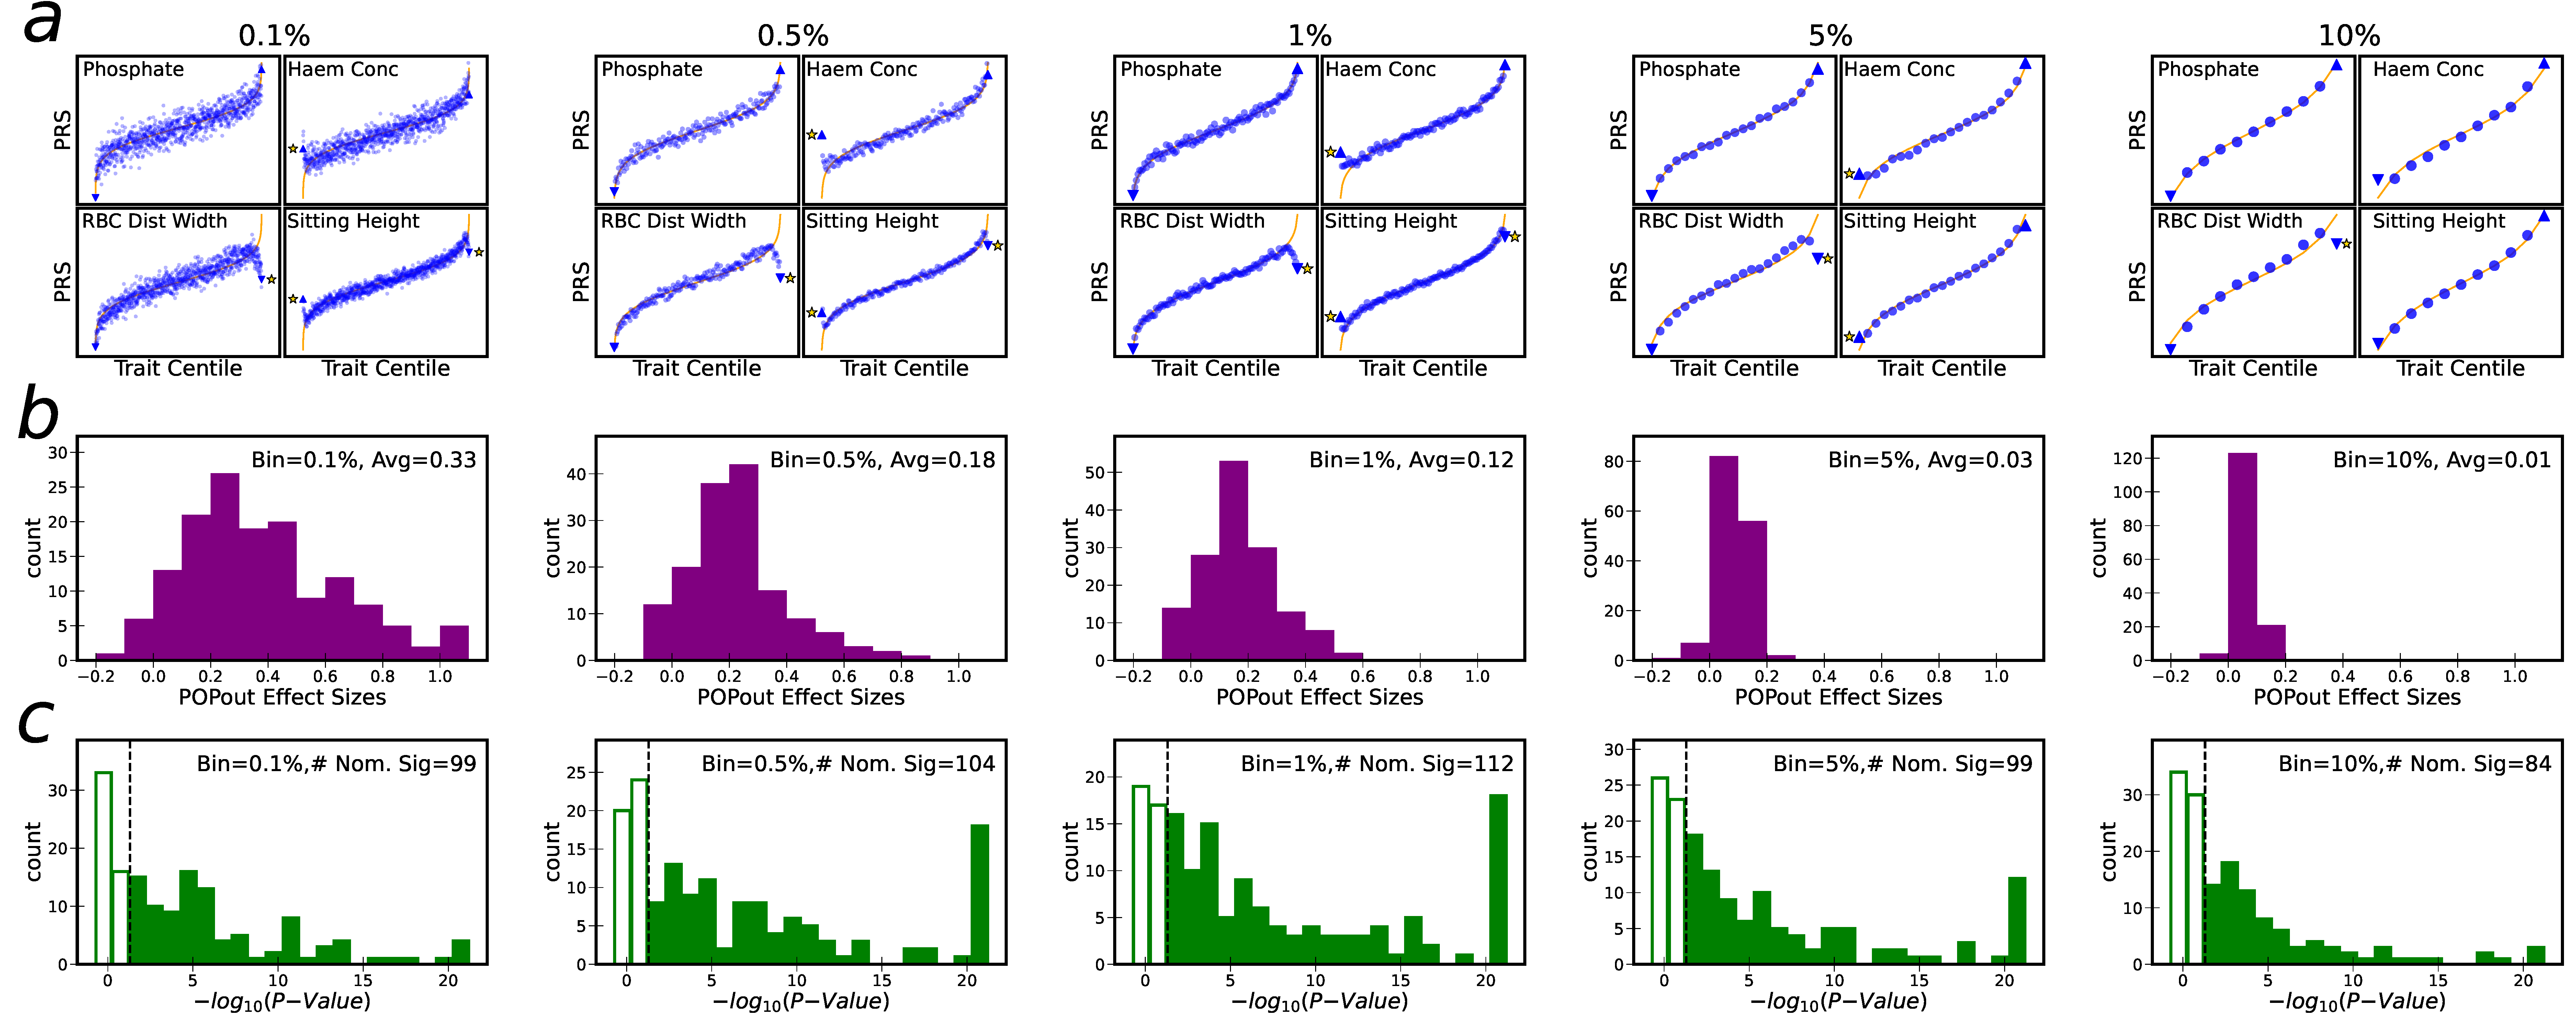
\includegraphics[trim=0cm 0cm 0cm 0cm, clip, width=\linewidth]{Figures/commonThresh.pdf} 
\caption{{{\bf Alternative POPout Thresholds (common variants)}
\textbf{a,} Index trait PRS-on-Phenotype plots for different POPout bin sizes: For bin sizes 
smaller than 1\%, POPout effect size is greater.  For bin sizes greater than 1\%, POPout 
is reduced, at 10\% nominally significant POPout (denoted with "*") exists only for RBC Dist. Width. 
\textbf{b,} The distribution of POPout effect sizes across all traits at difference bin sizes: Greater bin sizes reduces POPout effect. 
\textbf{b,} The distribution of POPout P-values across all traits at difference bin sizes: The number of significant P-values is maximized 
at 1\% due to a tradeoff between POPout signal (greater for small bins) and statistical power (greater for large bins). 
}} \label{sup_t1} \end{figure}
\FloatBarrier


\FloatBarrier \begin{figure}[!h] 
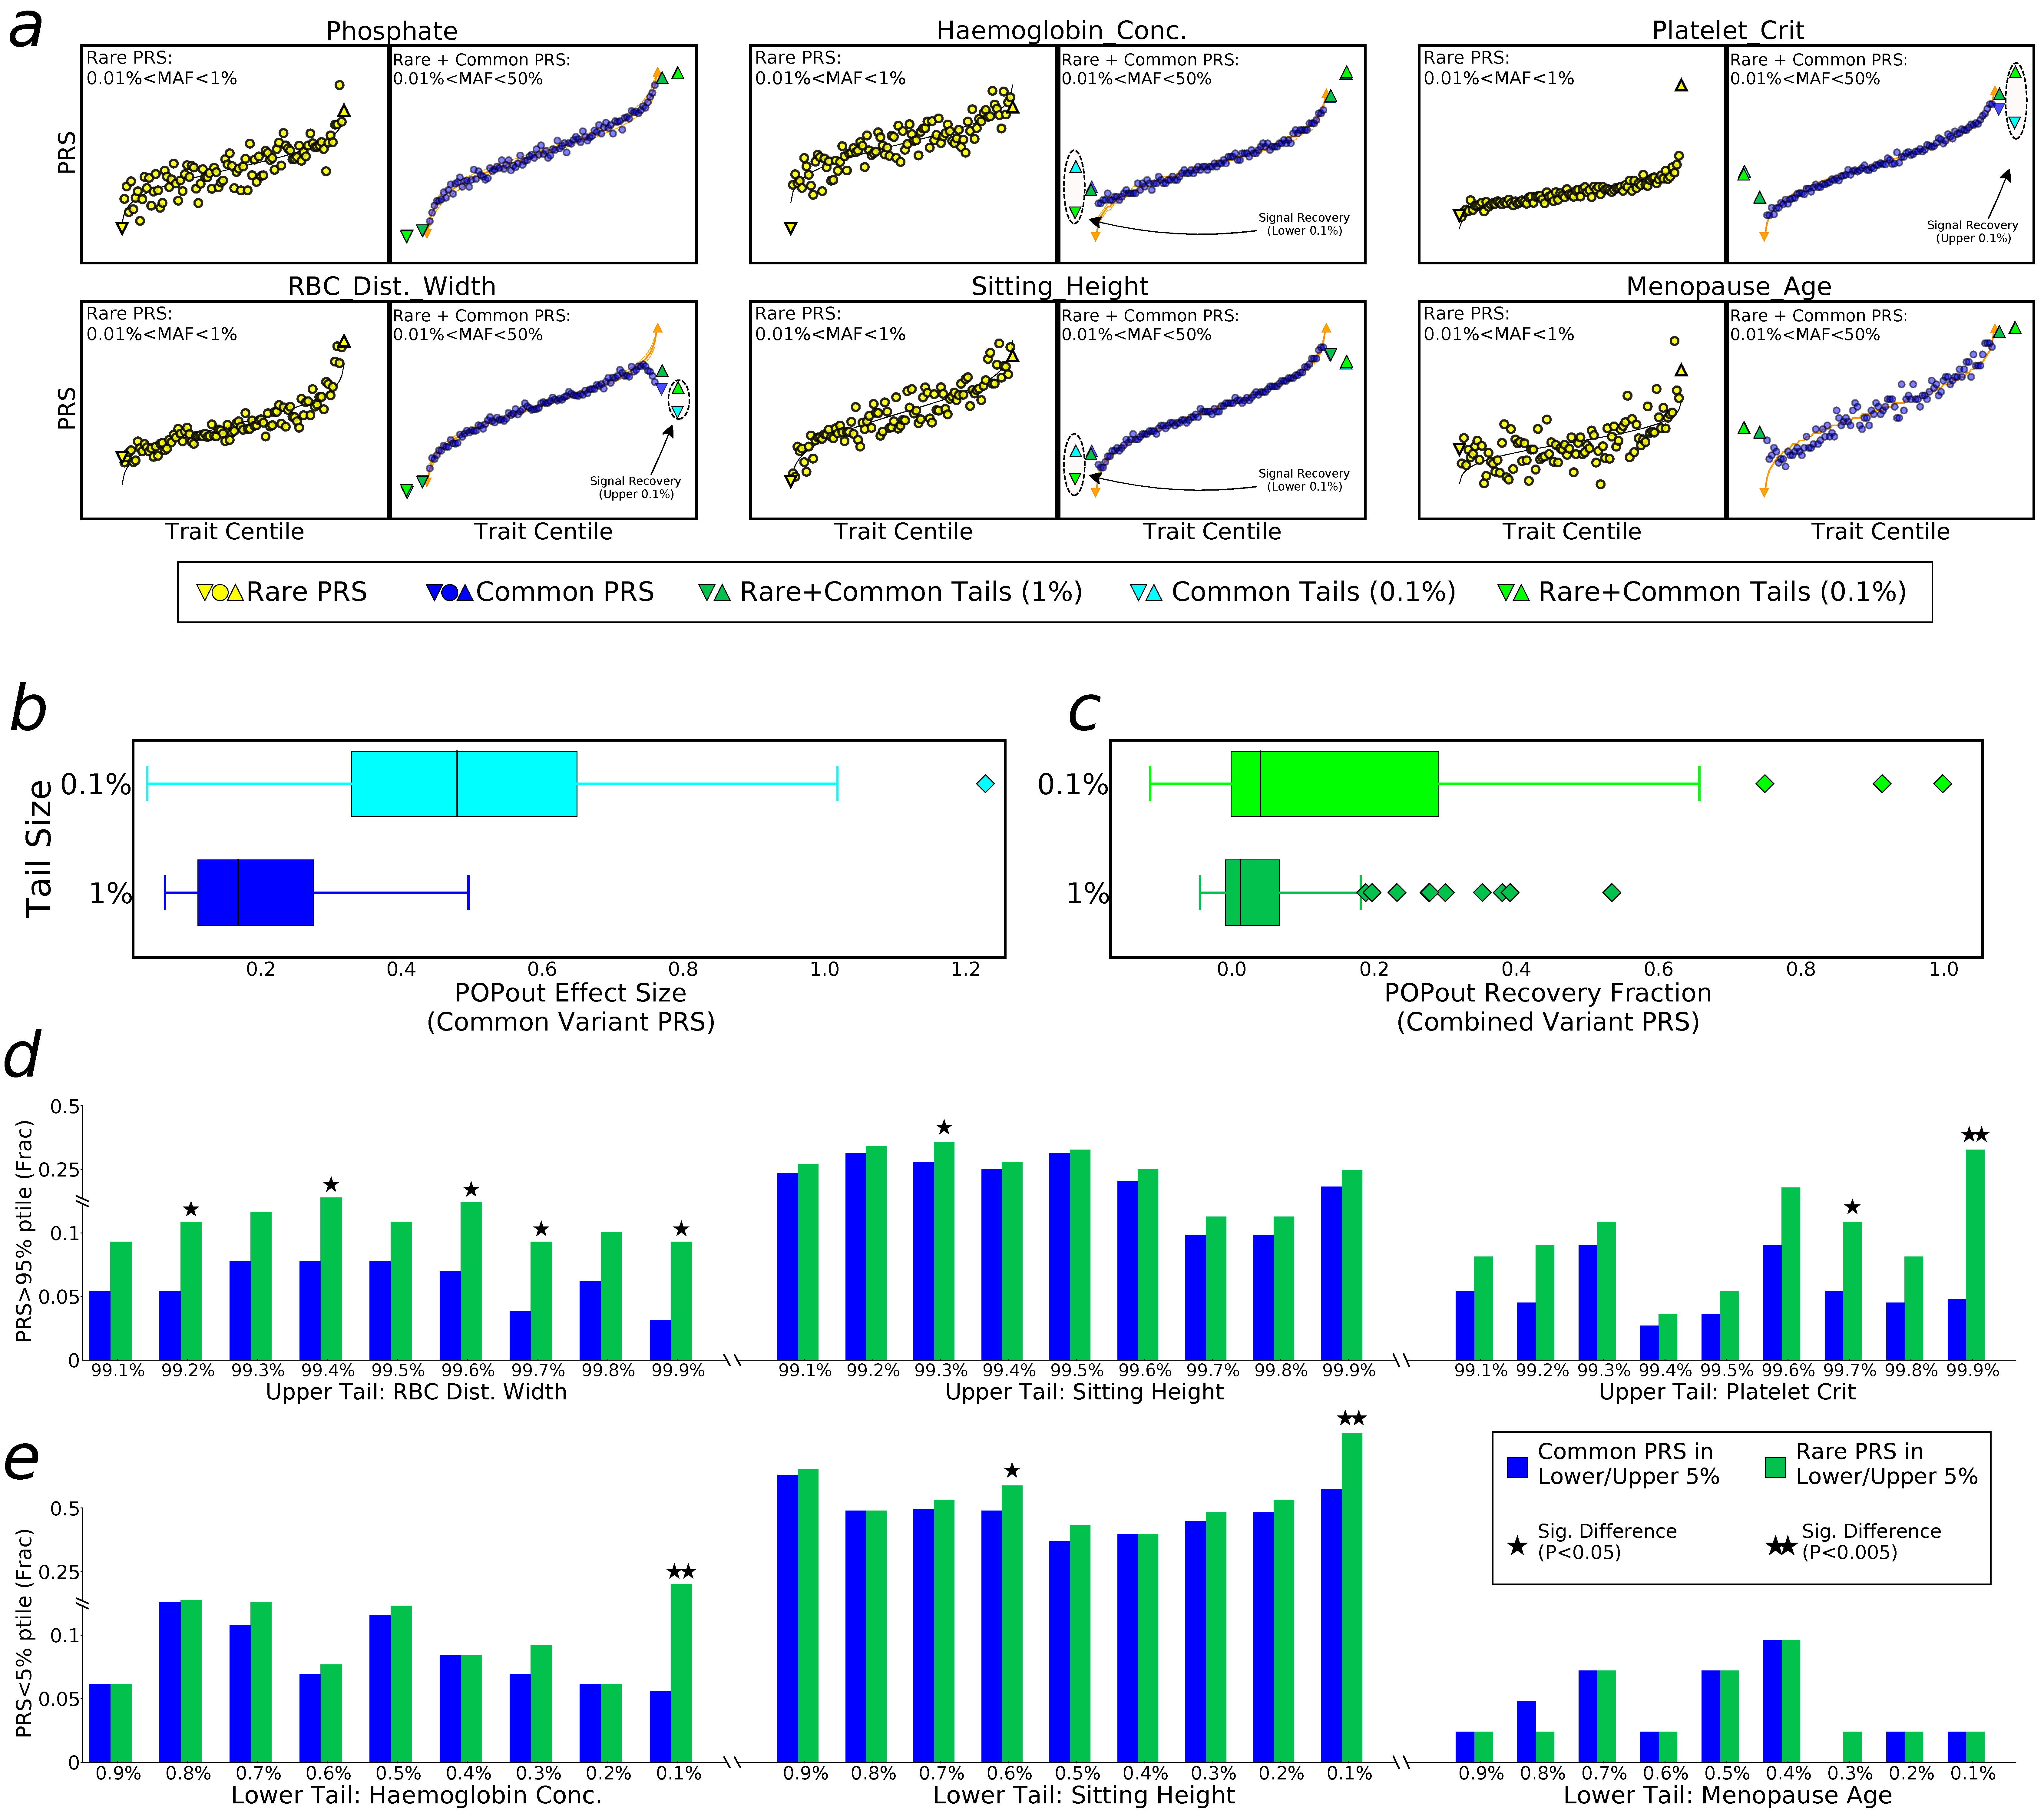
\includegraphics[trim=0cm 0cm 0cm 0cm, clip, width=\linewidth]{Figures/nexusSupplement.pdf} 
\caption{{{\bf Different POPout Thresholds for rare variants} 
\textbf{a,} PRS-on-Phenotype Plots that include the common and combined PRS means for the top and bottom 1\% and the top and bottom 0.1\% 
are shown for our four index traits and two other selected traits. 
\textbf{b,} Recovery of tail signal from combined PRS is varied.  For Heamolglobin the recovery is driven largely by the smallest bin. 
\textbf{c,} Restricting analysis to traits with FDR significant POPout and at least one rare variant, we see that POPout signals 
are significantly larger for the 0.1\% (P-val = 0.02) and recovery is significantly larger (P-val = 0.0005). 
}} \label{sup_t2} \end{figure}
\FloatBarrier
\clearpage \newpage 











































\FloatBarrier \begin{figure}[!h] 
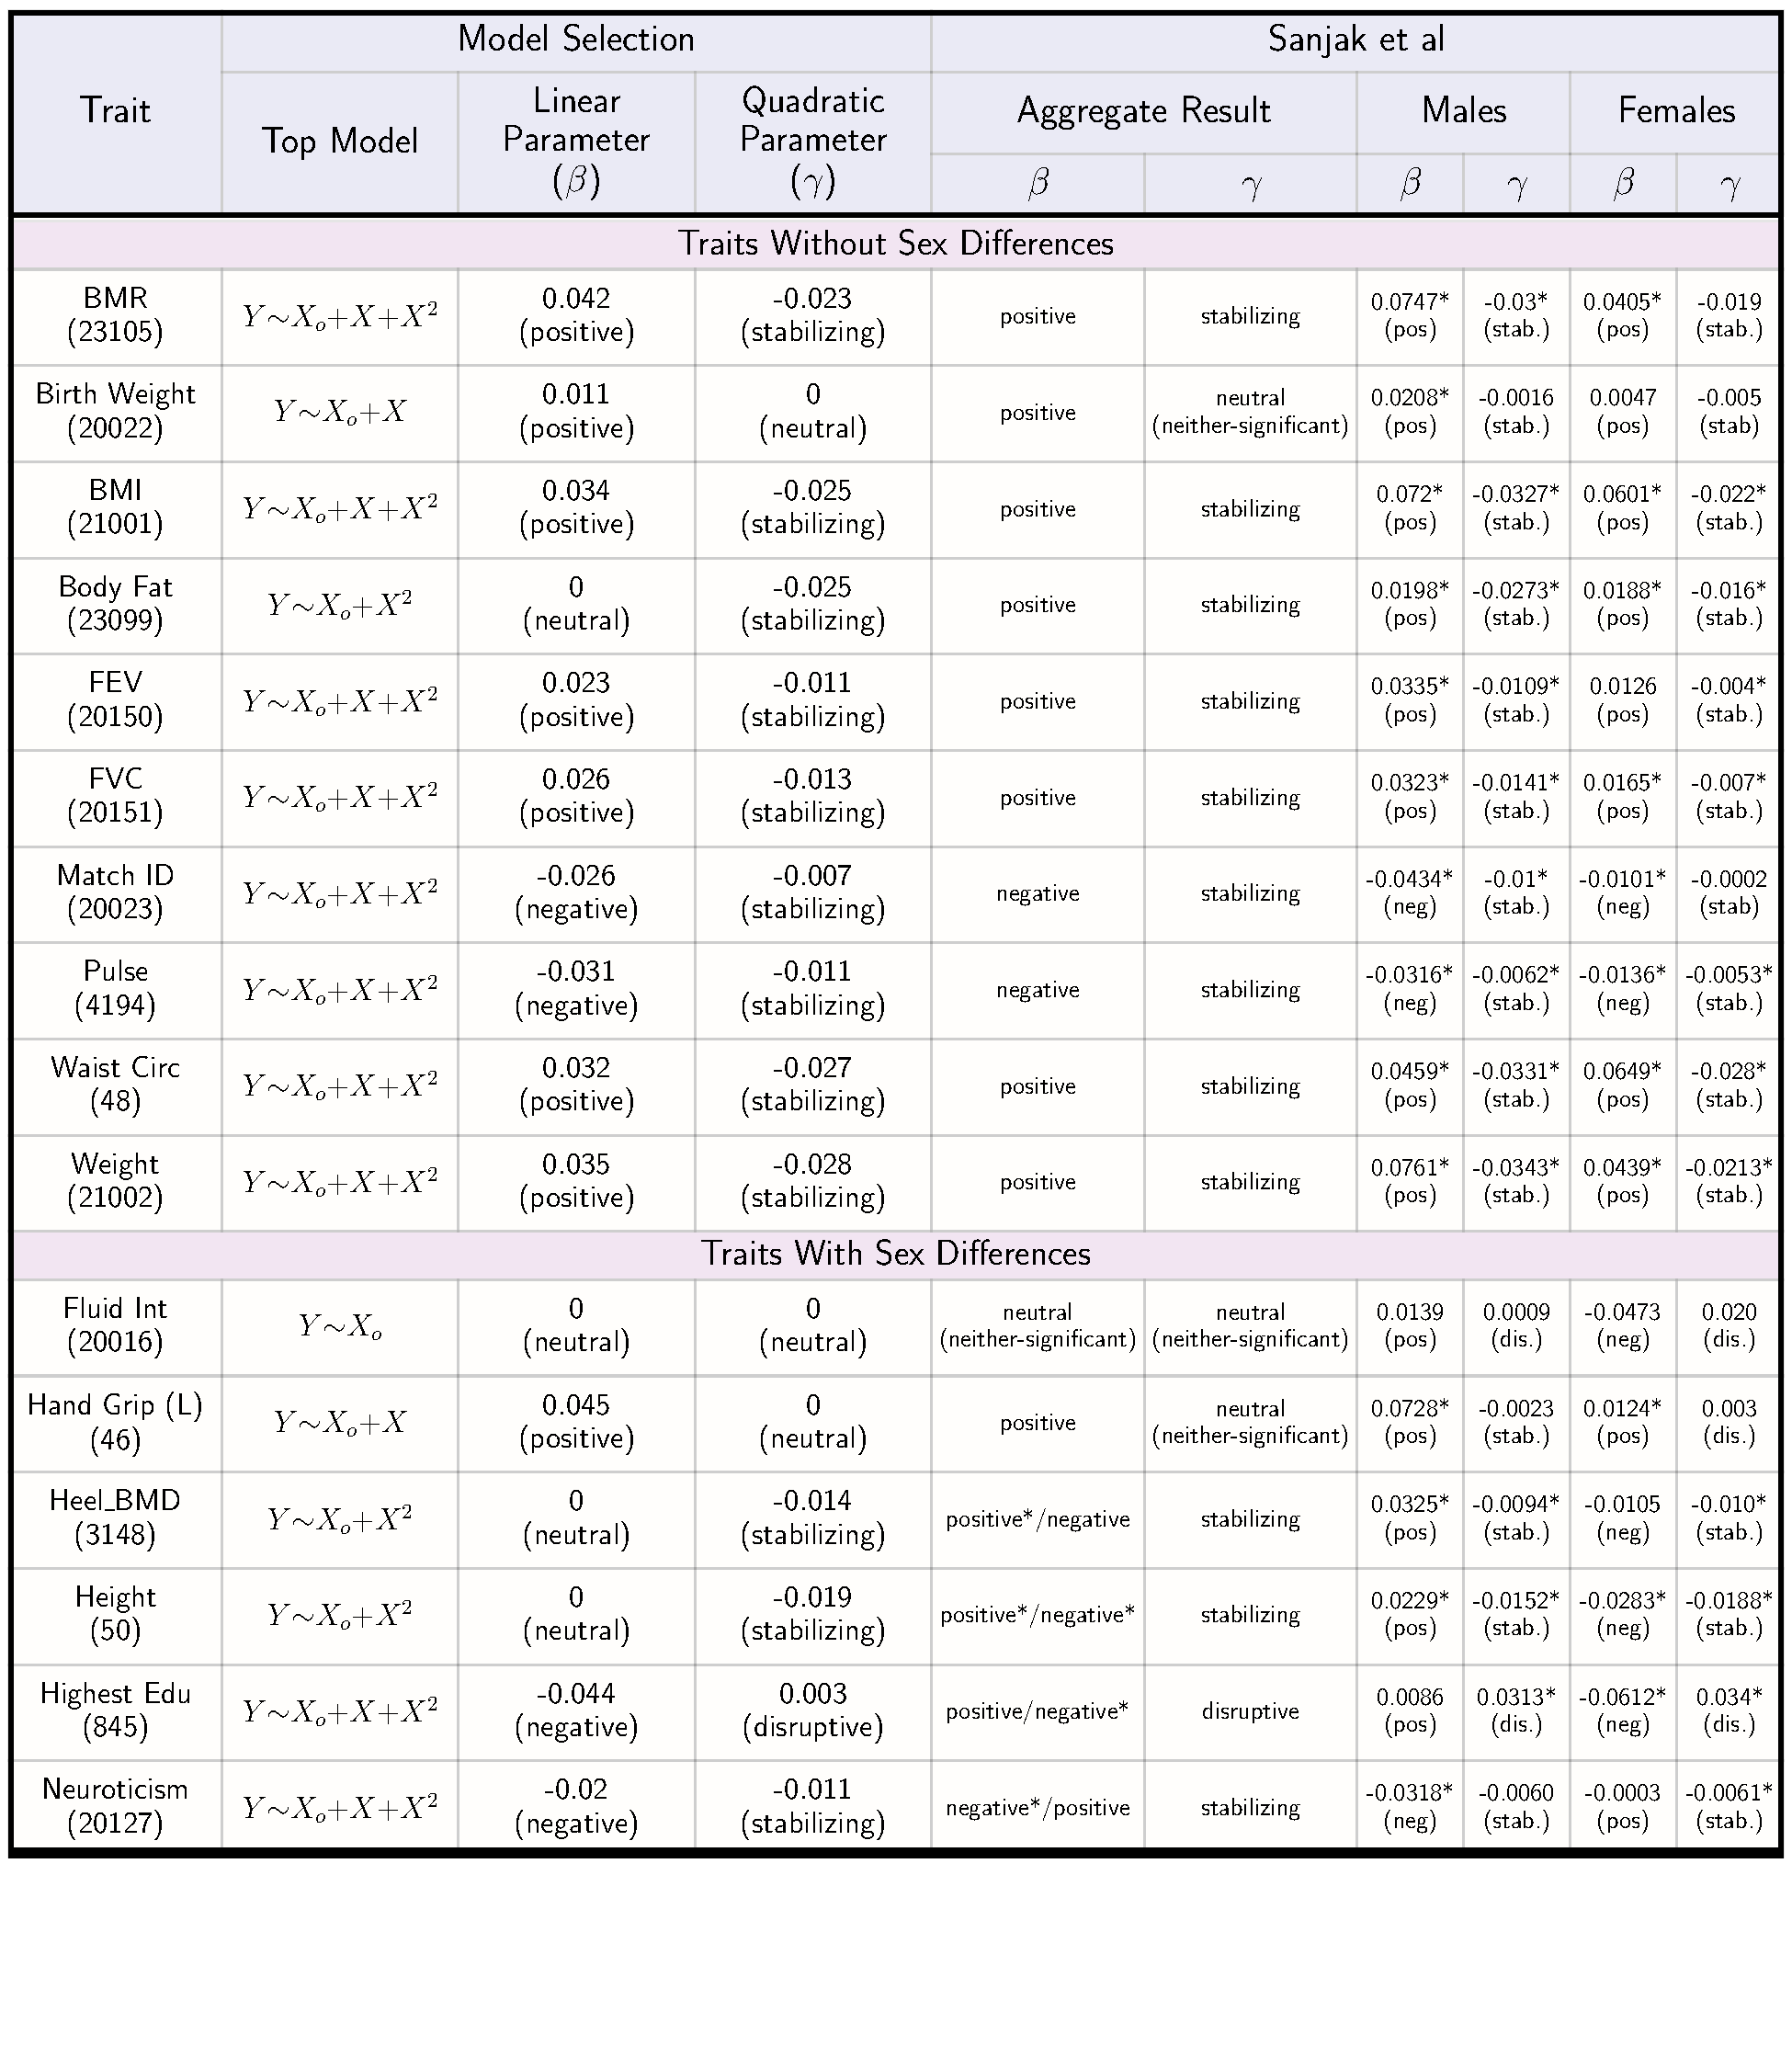
\includegraphics[trim=0cm 0cm 0cm 0cm, clip, width=\linewidth]{Figures/vishtable.pdf} 
\caption{{{\bf Replication of Lifetime Reproductive Success}
Comparing the overlapping traits without sex differences givens replication (i.e. statistically 
significant parameters included in our model) for 19 of 20 parameters (95\%), the only exception 
being \textit{Body Fat} where Sanjak et al reported a positive stabilizing result in both sexes 
while we selected a neutral stabilizing model. 
}} \label{sup_vish} \end{figure}
\FloatBarrier


\clearpage \newpage 





\clearpage \newpage 



\FloatBarrier \begin{figure}[!h] 
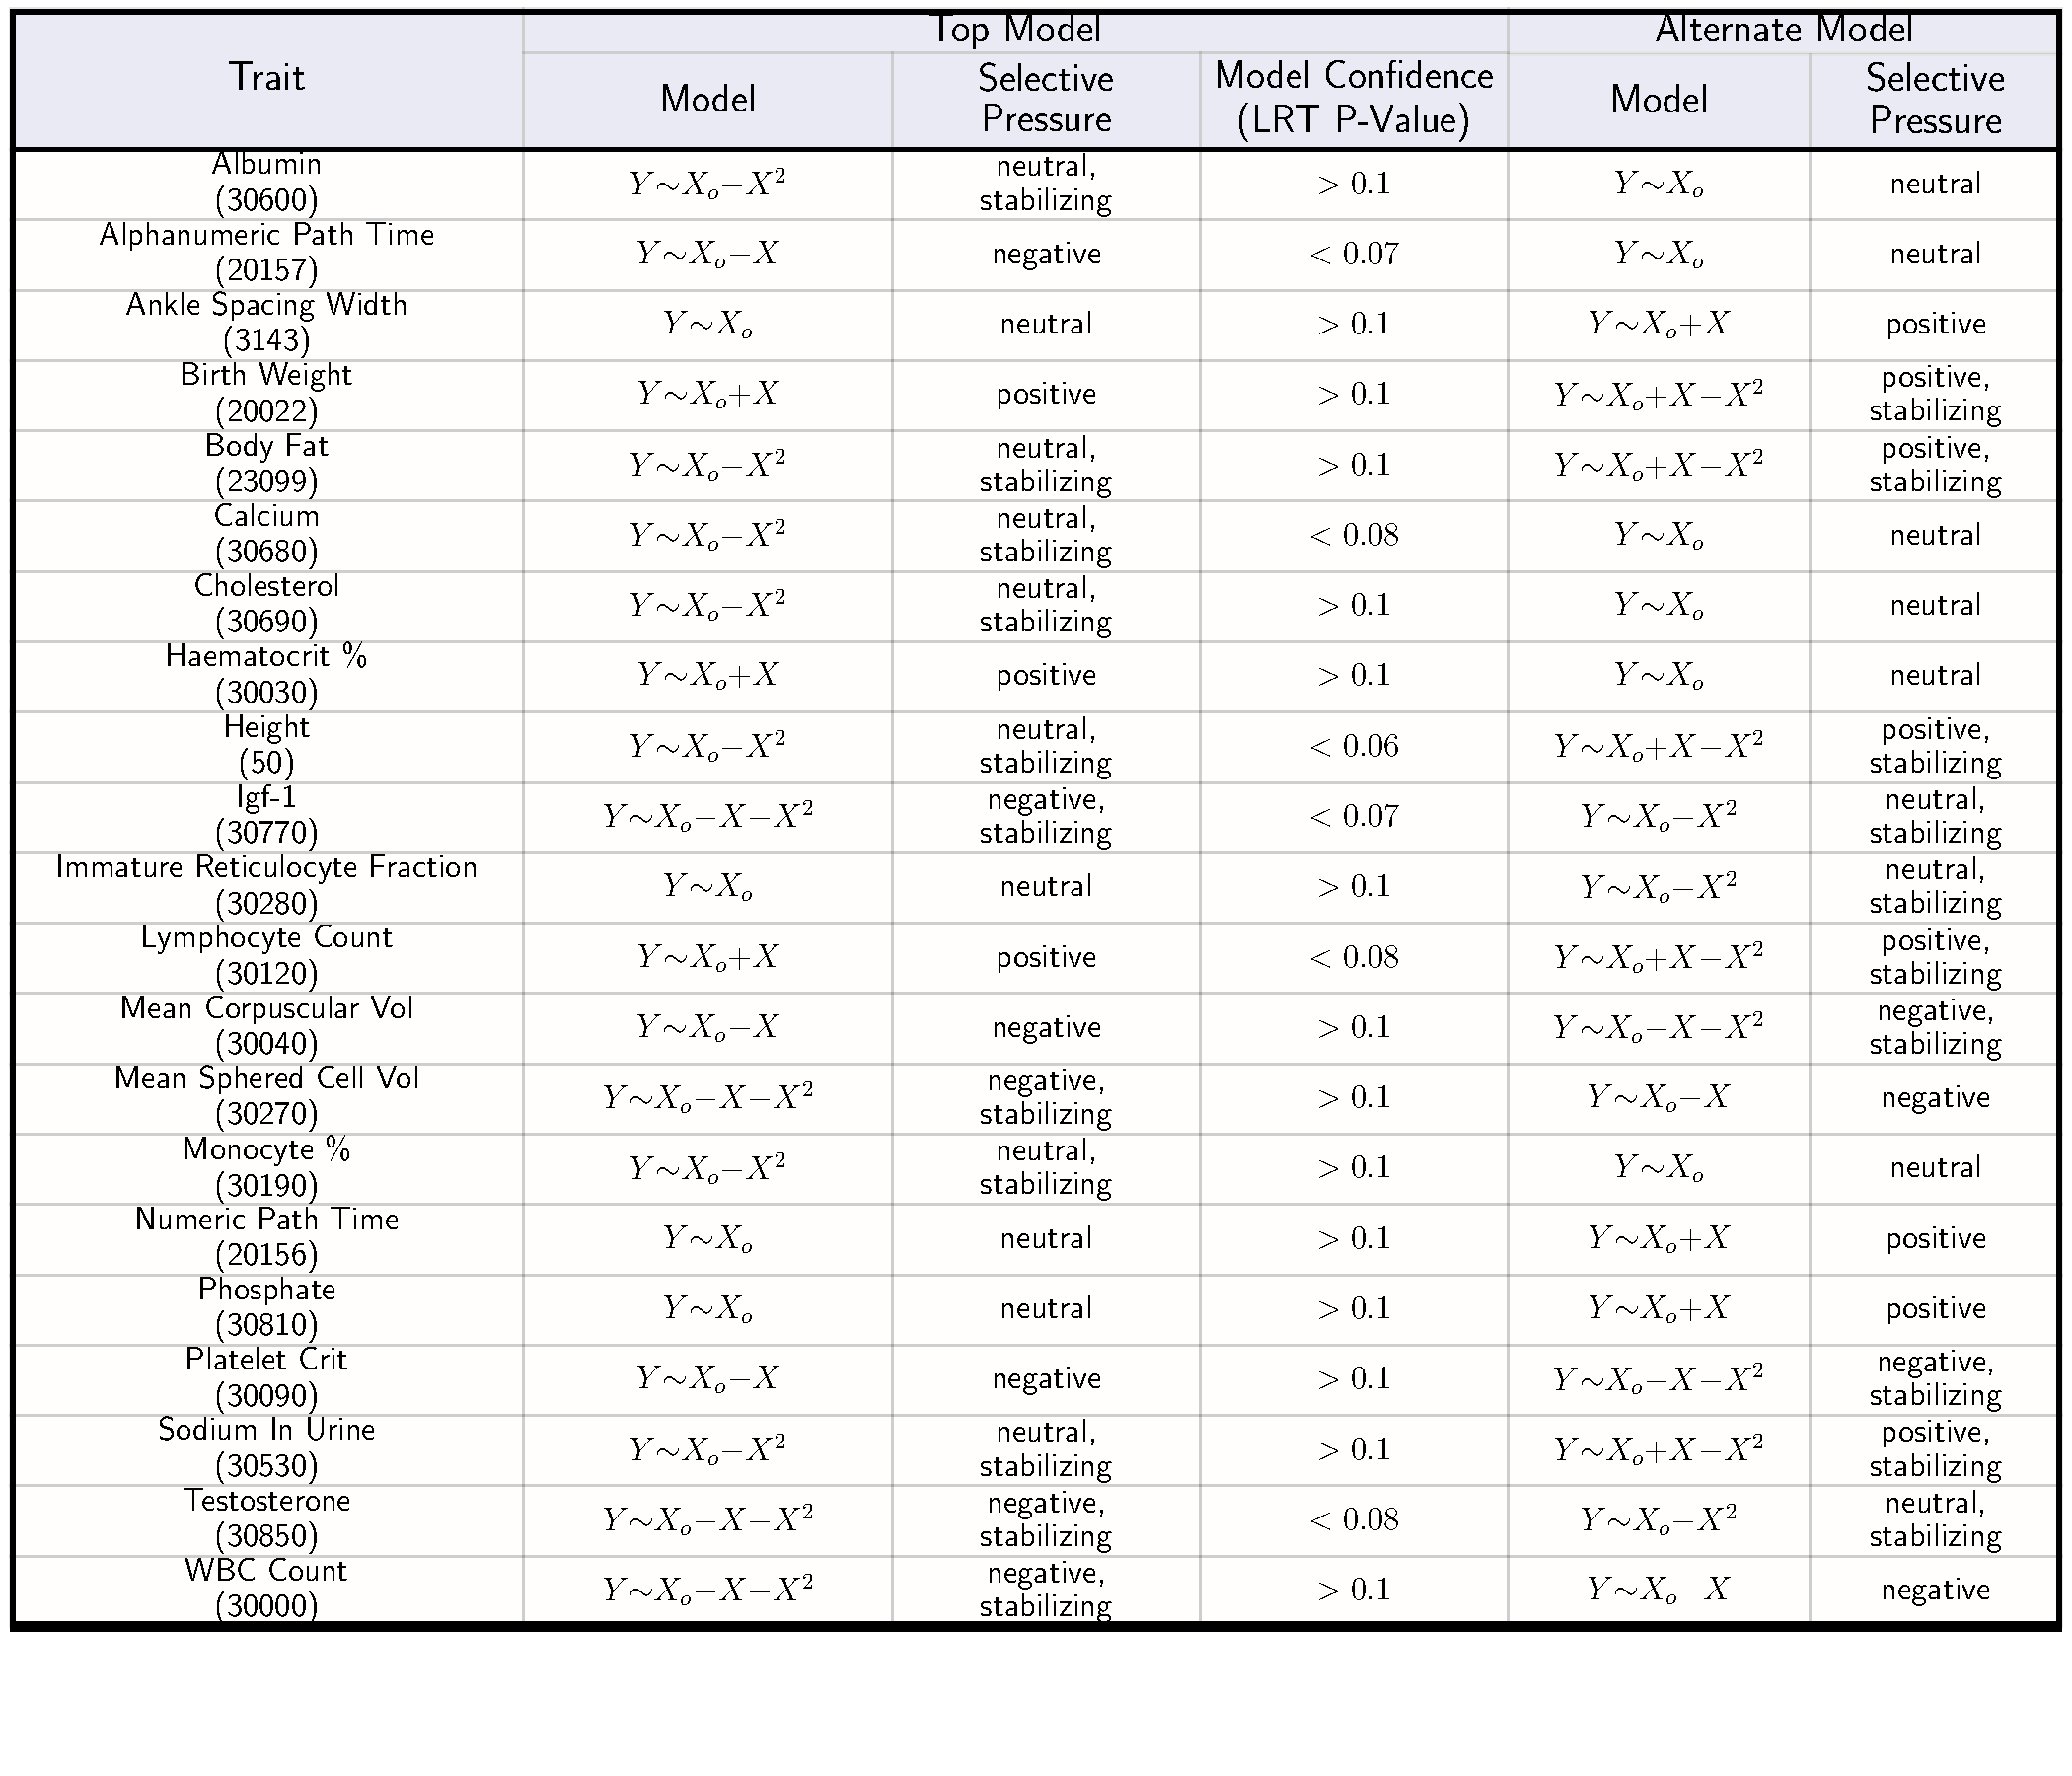
\includegraphics[trim=0cm 2.5cm 0cm 0cm, clip, width=\linewidth]{Figures/bictable.pdf} 
\caption{{
\footnotesize Model Selection - Sensitivity Analysis: In 21 of 74 traits, the top model 
selected using NIC was not significantly better than the alternate (next best) model 
at $\alpha=0.05$.  For these traits, the alternate model can be used.  Note that in most 
cases the alternate model does not drastically disagree with the top model. 
}} \label{sup_bic} \end{figure}
\FloatBarrier







\FloatBarrier \begin{figure}[!h] 
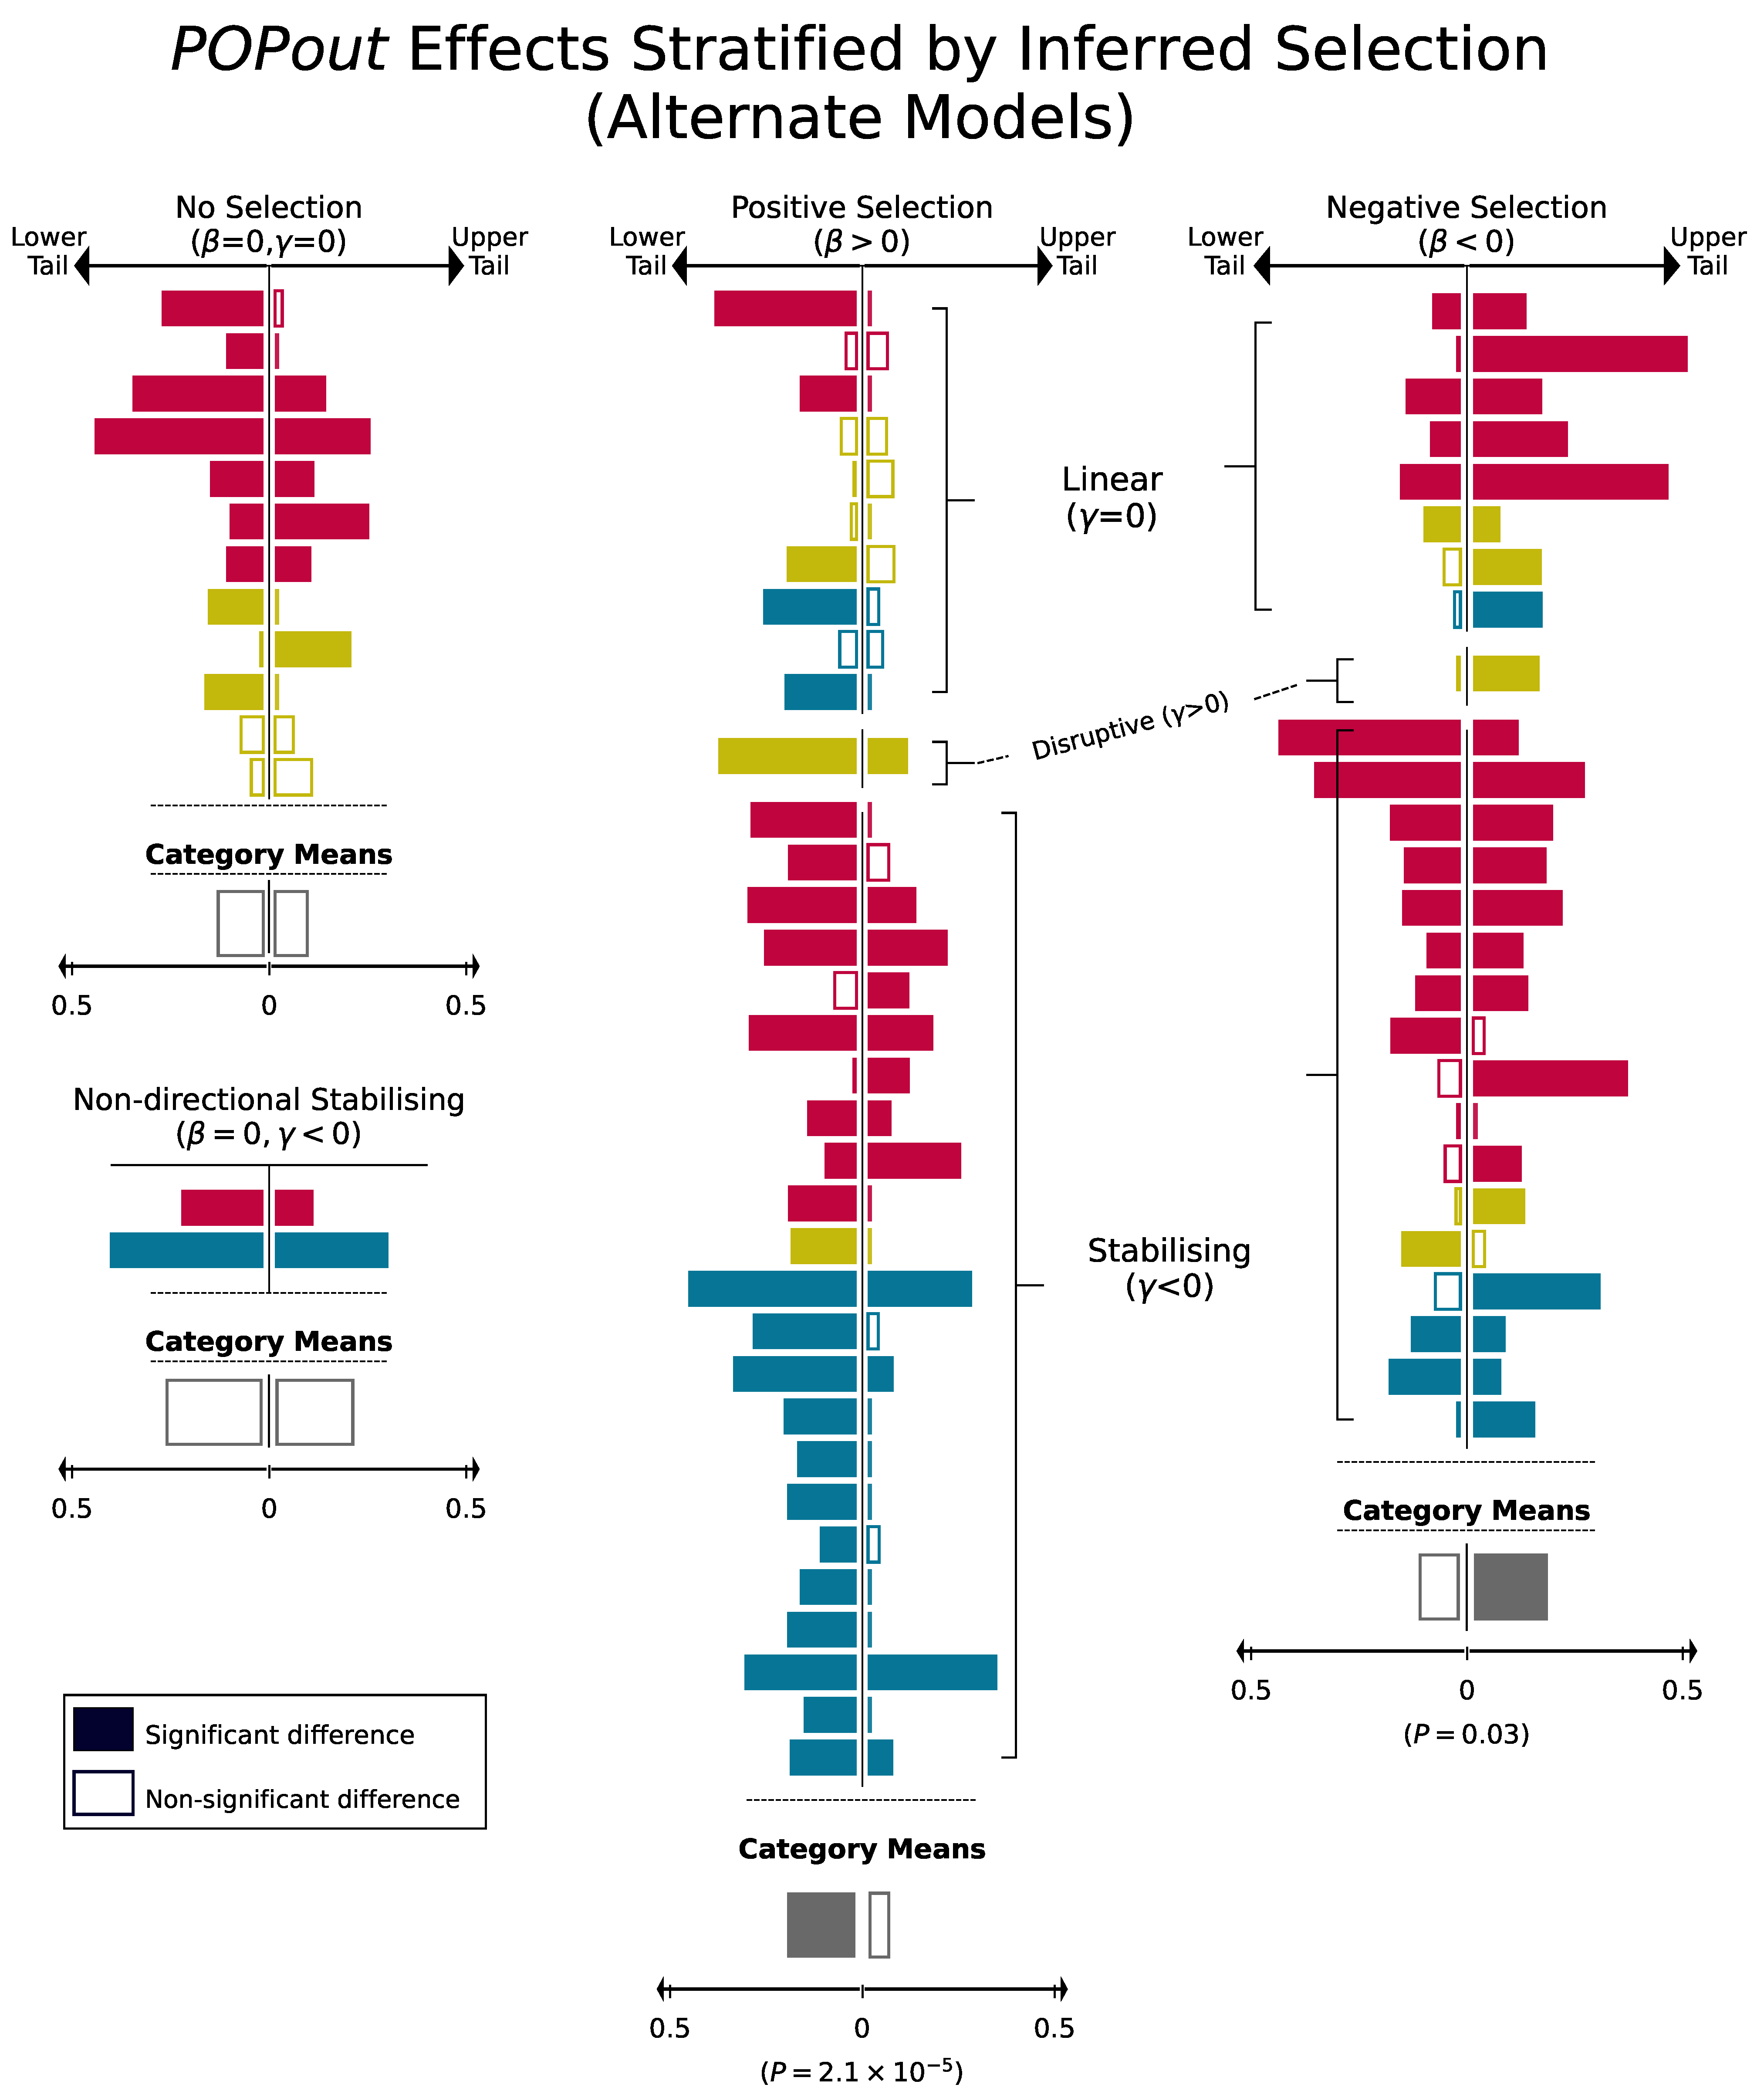
\includegraphics[trim=0cm 0cm 0cm 0cm, clip, width=\linewidth]{Figures/Fig4gAlt.pdf} 
\caption{{
\footnotesize Alternate Analysis: Compare to \fref{fig5}{g}.  Replacing Non-significant 
LRS models with alternate models reveals no significant difference in POPout tail effect sizes 
for neutral or non-directional stabilising selection, significantly larger lower tail effects are maintained 
for positive selection ($P=2.1 \times 10^{-5}$), and significantly larger upper tail effects are maintained for negative selection ($P=0.03$). 
}} \label{sup_evoAlt} \end{figure}
\FloatBarrier






\FloatBarrier \begin{figure}[!h] 
\includegraphics[trim=0cm 0cm 0cm 0cm, clip, width=0.75\linewidth]{Figures/cliveh2.pdf} 
\caption{{{\bf Estimating Unaccounted Heritability} 
TBD
}} \label{sup_clive_h2} \end{figure}
\FloatBarrier


\FloatBarrier \begin{figure}[!h] 
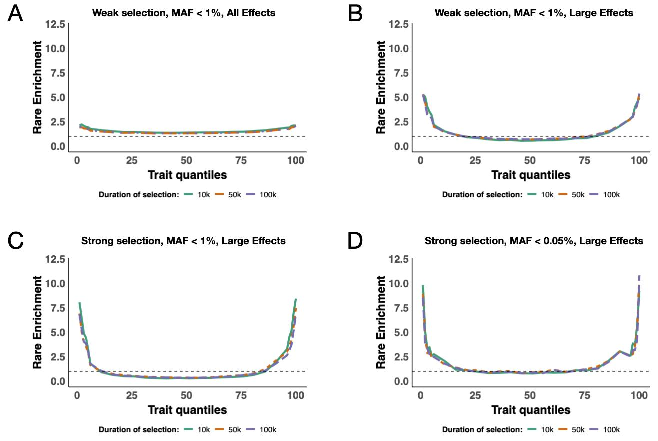
\includegraphics[trim=0cm 0cm 0cm 0cm, clip, width=0.75\linewidth]{Figures/sup_anil1.pdf} 
\caption{{{\bf Rare variants are similarly enriched in the trait tails across longer durations of stabilising selection.}
Enrichment of rare alleles in simulations under weak and strong selection scenarios, stratified by rare variant classification and effect size. For each stratification (A-D), rare variant enrichment is shown across trait quantiles for different durations of stabilising selection (i.e. 10k (green), 50k (orange), and 100k (purple) generations of selection). We observe no major differences in rare variant enrichments between timepoints. The dotted horizontal line represents enrichment under neutrality.
}} \label{sup_anil1} \end{figure}
\FloatBarrier













\FloatBarrier \begin{figure}[!h] 
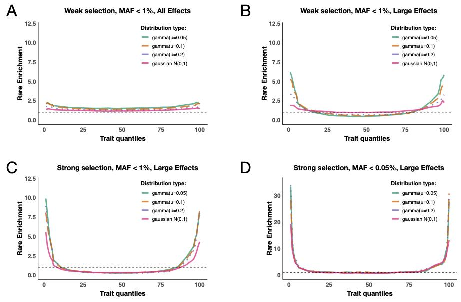
\includegraphics[trim=0cm 0cm 0cm 0cm, clip, width=0.75\linewidth]{Figures/sup_anil2.pdf} 
\caption{{{\bf Rare variants are enriched in the trait tails across different mutation distributions} 
Enrichment of rare alleles in simulations under weak and strong selection scenarios, stratified by rare variant classification and effect size. For each stratification (A-D), rare variant enrichment is shown across trait quantiles for different type of mutation distributions: gamma (mean=0.05, shape= 0.186) in green, gamma (mean=0.1, shape= 0.186) in orange, gamma (mean=0.2, shape= 0.186) in purple, and gaussian N(0,1) in pink. For each stratification, we observe rare variant enrichment in the tails after 1N generations of stabilising selection with slight differences in the degree of enrichment depending on the distribution. All three heavy-tailed gamma distributions produced greater enrichment of rare variants in the tails than the gaussian distribution. The dotted horizontal line represents enrichment under neutrality.
}} \label{sup_anil2} \end{figure}
\FloatBarrier


\FloatBarrier \begin{figure}[!h] 
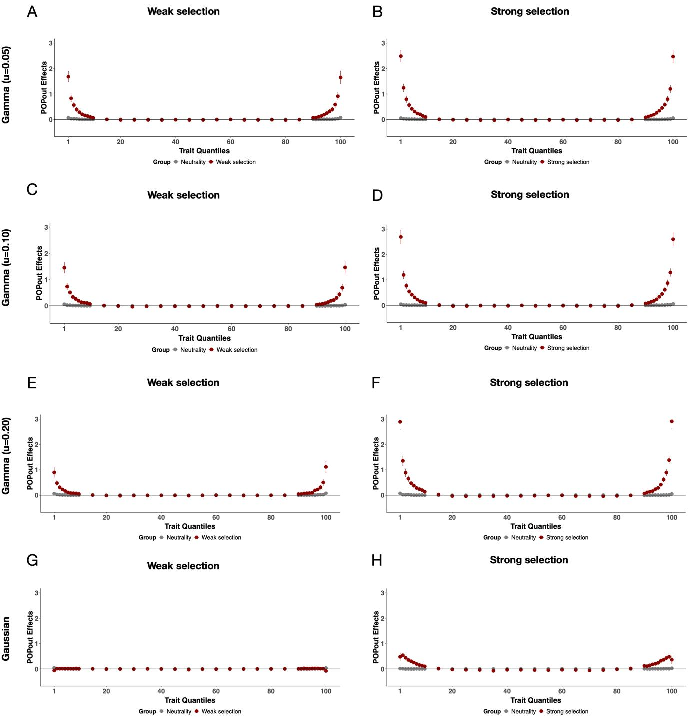
\includegraphics[trim=0cm 0cm 0cm 0cm, clip, width=\linewidth]{Figures/sup_anil3.pdf} 
\caption{{{\bf POPout effects are observed under different mutation distributions.}
POPout effects are shown across trait quantiles averaged over 100 simulations (mean and CIs shown) under neutrality (in grey) and (weak/strong) selection (in red). Results are visualized stratified by mutation distribution: gamma (mean=0.05, shape= 0.186) in A/B, gamma (mean=0.1, shape= 0.186) in C/D, gamma (mean=0.2, shape= 0.186) in E/F, and gaussian N(0,1) in G/H. Selection was introduced for 1N generations. We observe strong POPout effects in the tail across different gamma distributions and strengths of selection. For the gaussian, we only observe POPout effects under strong selection.
}} \label{sup_anil3} \end{figure}
\FloatBarrier

























\clearpage \newpage
\section*{Supplementary Tables} \label{sec:supplement}

\renewcommand{\figurename}{Supplementary Table}
\setcounter{figure}{0}
\FloatBarrier 
\begin{figure}[!h] 
\includegraphics[trim=0cm 0cm 0cm 0cm, clip, width=\linewidth]{Figures/sup0.1.pdf} 
\caption{{\textbf{Traits 1-25}}} \label{sup2a} \end{figure} \FloatBarrier


\setcounter{figure}{0}
\FloatBarrier 
\begin{figure}[!h] 
\includegraphics[trim=0cm 0cm 0cm 0cm, clip, width=\linewidth]{Figures/sup0.2.pdf} 
\caption{{\textbf{Traits 25-50}}} \label{sup2b} \end{figure} \FloatBarrier


\setcounter{figure}{0}
\FloatBarrier 
\begin{figure}[!h] 
\includegraphics[trim=0cm 0cm 0cm 0cm, clip, width=\linewidth]{Figures/sup0.3.pdf} 
\caption{{\textbf{Traits 50-74}}} \label{sup2c} \end{figure} \FloatBarrier

%
%
%
%
%
\clearpage \newpage
\end{document}





